\documentclass[journal]{IEEEtran}

\usepackage{amsmath,amssymb,amsfonts}
\usepackage{algorithmic}
\usepackage{graphicx}
\usepackage{textcomp}
\usepackage{cite}
\usepackage{booktabs}
\usepackage{microtype}
\usepackage{url}
\usepackage{multirow}
\usepackage{array}
\usepackage{xcolor}

\graphicspath{{../figuras/}}

\setlength{\textfloatsep}{5.5pt plus 1pt minus 1.5pt}
\setlength{\floatsep}{4.5pt plus 1pt minus 1.5pt}
\setlength{\dbltextfloatsep}{6.0pt plus 1pt minus 1.5pt}
\setlength{\dblfloatsep}{5.0pt plus 1pt minus 1.5pt}

\begin{document}

\title{Predictive Distributed Workload Orchestration via Optical Inter-Satellite Links for Thermal-Energy Balancing in Orbital Data Center Constellations}

\author{Dafnh\^{e}~Thor~Castro~de~Martins~Barros~and~Fl\'{a}vio~Barcelos~Braz~da~Silva%
\thanks{D. T. C. M. Barros and F. B. B. da Silva are with the Graduate Program in Control and Automation Engineering (PROPECAUT), Federal Institute of Esp\'{i}rito Santo (IFES), Serra, ES, 29173-087, Brazil (e-mail: dafnhe.thor@msn.com; flavio.silva@ifes.edu.br).}}

\markboth{}%
{Barros and Silva: Predictive Distributed Workload Orchestration via OISL for Orbital Data Centers}

\maketitle

\begin{abstract}
Transferring heavy Artificial Intelligence (AI) and scientific computing workloads to space-based orbital data centers (ODCs) has emerged as a disruptive paradigm to circumvent terrestrial electrical grid congestion, land constraints, and millions of liters of evaporative cooling water consumption. However, operating dense computing clusters in Low Earth Orbit (LEO) introduces severe multi-physical vulnerabilities: during periodic planetary shadow transits ($35.63$~min per $95.65$-min revolution at $550$~km altitude), isolated spacecraft must sustain hundred-kilowatt computing loads entirely through electrochemical Battery Energy Storage Systems (BESS). This severe cycling causes deep discharge (Depth-of-Discharge $> 50\%$) and extreme thermal swings, triggering accelerated lithium-ion capacity loss under Arrhenius degradation laws and restricting operational lifetime to barely $3.1$~years. To address these fundamental physical constraints, this paper establishes a cooperative orbital constellation architecture governed by predictive distributed workload migration via high-capacity Coherent Optical Inter-Satellite Links (OISL). We formulate a Distributed Predictive Multi-Agent Model Predictive Control (D-PMPC) framework that anticipates orbital illumination transitions over a receding horizon, proactively shunting batch training workloads from eclipsed satellites to sunlit peer nodes possessing surplus photovoltaic generation. The optimization problem couples orbital beta-angle dynamics, non-linear Stefan-Boltzmann radiative cooling, and electrochemical battery degradation, solved in real time via the Alternating Direction Method of Multipliers (ADMM). Numerical simulations across a 32-node Walker-Delta constellation ($h = 550$~km, $i = 53^\circ$) evaluated over 30 consecutive orbital revolutions ($47.82$~h, $17,218$~integration steps per spacecraft) demonstrate the feasibility of cooperative D-PMPC in sustaining limit-cycle stability with zero secular drift ($0.0000\%$, $SoC_{min} \approx 80.37\%$), reducing battery Depth-of-Discharge by $65.4\%$ (from $52.0\%$ to $18.0\%$), confining silicon junction temperatures below $74.0^\circ$C (mitigating thermal fatigue by $51.2\%$), increasing global solar harvesting efficiency to $96.8\%$, and extending projected battery calendar life from $3.1$ to $11.8$~years ($+280.6\%$ extension), while incurring an optical communication latency overhead of only $215$~ms.
\end{abstract}

\begin{IEEEkeywords}
Orbital data centers, optical inter-satellite links (OISL), distributed model predictive control (D-MPC), battery degradation, Stefan-Boltzmann radiative cooling, space computing, LEO constellations.
\end{IEEEkeywords}

\vspace{0.8ex}
\noindent\small{\textbf{\textit{Resumo}}---A transfer\^{e}ncia de cargas computacionais pesadas de Intelig\^{e}ncia Artificial (IA) para centros de dados orbitais (ODCs) surge como um paradigma disruptivo para mitigar a satura\c{c}\~{a}o das redes el\'{e}tricas terrestres e o consumo de milh\~{o}es de litros de \'{a}gua para resfriamento evaporativo. Contudo, a opera\c{c}\~{a}o de clusters computacionais densos em \'{O}rbita Baixa da Terra (LEO) enfrenta severas vulnerabilidades multif\'{i}sicas: durante o eclipse planet\'{a}rio peri\'{o}dico ($35,63$~min por revolu\c{c}\~{a}o de $95,65$~min a $550$~km de altitude), sat\'{e}lites isolados precisam sustentar cargas de centenas de quilowatts exclusivamente por meio de sistemas de baterias eletroqu\'{i}micas (BESS). Esse regime c\'{i}clico severo imp\~{o}e descargas profundas (DoD $> 50\%$) e intensas oscila\c{c}\~{o}es t\'{e}rmicas, acelerando a perda de capacidade regida por leis cin\'{e}ticas de Arrhenius e limitando a vida \'{u}til a apenas $3,1$~anos. Para mitigar esses limites f\'{i}sicos, este artigo introduz uma arquitetura de constela\c{c}\~{a}o cooperativa governada por migra\c{c}\~{a}o preditiva de carga via Enlaces Laser \'{O}pticos Inter-Sat\'{e}lite (OISL). Formula-se um algoritmo de Controle Preditivo Baseado em Modelos Distribu\'{i}do Multi-Agente (D-PMPC) que antecipa as transi\c{c}\~{o}es de ilumina\c{c}\~{a}o ao longo de um horizonte m\'{o}vel, transferindo tarefas de treinamento de sat\'{e}lites eclipsados para sat\'{e}lites iluminados com excedente fotovoltaico. O problema acopla a din\^{a}mica do \^{a}ngulo beta, radia\c{c}\~{a}o t\'{e}rmica de Stefan-Boltzmann e degrada\c{c}\~{a}o de baterias, resolvido via ADMM. Simula\c{c}\~{o}es em uma constela\c{c}\~{a}o Walker-Delta de 32 n\'{o}s ao longo de 30 revolu\c{c}\~{o}es orbitais consecutivas ($47,82$~h, $17.218$~passos de integra\c{c}\~{a}o) demonstram a viabilidade e a estabilidade do ciclo limite com deriva secular nula ($0,0000\%$), indicam uma redu\c{c}\~{a}o do DoD em $65,4\%$ (de $52,0\%$ para $18,0\%$), cont\^{e}m a temperatura de jun\c{c}\~{a}o abaixo de $74,0^\circ$C, elevam a efici\^{e}ncia de capta\c{c}\~{a}o solar para $96,8\%$ e ampliam a vida \'{u}til projetada da bateria de $3,1$ para $11,8$~anos ($+280,6\%$), com lat\^{e}ncia de apenas $215$~ms.}

\vspace{0.8ex}
\noindent\small{\textbf{\textit{Palavras-chave}}---Centros de dados orbitais, enlaces \'{o}pticos inter-sat\'{e}lite (OISL), controle preditivo distribu\'{i}do (D-MPC), degrada\c{c}\~{a}o de baterias, resfriamento radiativo de Stefan-Boltzmann, computa\c{c}\~{a}o espacial, constela\c{c}\~{o}es LEO.}

\section{Introduction}
\IEEEPARstart{T}{he} exponential scale-up of deep neural networks, large foundation models, and autonomous planetary Earth observation data processing has driven global data center electrical consumption and water footprints to critical limits \cite{barroso2019datacenter, bloch2026earth}. Modern terrestrial hyperscale data centers frequently demand electrical power capacities between $100\text{ MW}$ and $1\text{ GW}$, placing unprecedented strains on regional power transmission grids, consuming billions of liters of potable water annually for evaporative cooling towers, and generating substantial carbon emissions \cite{bloch2026earth, liu2015greening}. In response to these terrestrial infrastructure bottlenecks, space-based computing and Orbital Data Centers (ODCs) operating in Low Earth Orbit (LEO) have emerged as an attractive frontier across aerospace and computer engineering \cite{aguera2025towards, turyshev2026orbital, bleier2023space}. In the orbital vacuum, high-density solar arrays capture continuous extraterrestrial Air Mass Zero (AM0) solar irradiance ($S_0 \approx 1361.0\text{ W/m}^2$) uninhibited by atmospheric attenuation, weather cycles, or day-night diurnal boundaries \cite{kopp2011new, wertz2011space}. Furthermore, thermal dissipation requires zero water, relying exclusively on radiative infrared emission directly into deep space \cite{gilmore2002spacecraft}.

Despite these theoretical advantages, operating multi-kilowatt to hundred-kilowatt high-performance computing (HPC) payloads on autonomous, standalone LEO satellites introduces severe astrodynamical, thermal, and electro-chemical bottlenecks \cite{turyshev2026orbital, denby2020orbital, kim2025gpu}. In a circular LEO orbit at an altitude of $h = 550.0\text{ km}$, a satellite completes an orbital revolution every $\tau \approx 5,738.99\text{ s} \approx 95.65\text{ min}$ ($\approx 15.05\text{ orbits/day}$), spending roughly $60.02\text{ min}$ under solar illumination and $35.63\text{ min}$ traversing the Earth's umbra shadow cone (eclipse) \cite{curtis2014orbital, patel2005spacecraft}. During eclipse, photovoltaic generation drops abruptly to zero. If an isolated satellite sustains an uncoordinated computing load of $100\text{ kW}$ during shadow, its Battery Energy Storage System (BESS) must deliver the entire electrical power demand ($105\text{ kW}$ including platform bus) \cite{patel2005spacecraft, li2024battery}. Accounting for discharge conversion efficiency ($\eta_{dis} = 0.96$), this drives the cyclic Depth-of-Discharge (DoD) to $52.0\%$, inducing severe mechanical micro-cracking, lithium plating, and solid electrolyte interphase (SEI) growth governed by non-linear Arrhenius degradation kinetics \cite{wang2011cycle, xu2018modeling}. Under such intense cyclic stress, state-of-the-art LiFePO4 or NMC battery cells degrade to their $80\%$ End-of-Life (EOL) capacity threshold within only $17,038\text{ cycles}$ ($3.10\text{ years}$), severely undermining the economic viability of multi-million-dollar space assets \cite{turyshev2026orbital, leyva2023satellite}.

Simultaneously, thermal management in space presents an equally daunting challenge. In the hard vacuum of LEO, convective heat exchange is non-existent; all heat generated by high-power processing silicon must be rejected via thermal radiation governed by the Stefan-Boltzmann law ($q_{rad} \propto \epsilon \sigma T^4$) \cite{gilmore2002spacecraft, skadron2004temperature}. Dissipating $100\text{ kW}$ of compute heat while entering eclipse induces steep temperature gradients across structural radiators and silicon chip packages, accelerating solder joint thermomechanical fatigue and threatening semiconductor junction integrity whenever $T_j > 85.0^\circ\text{C}$ \cite{bartolini2013thermal, felix2024total, lentaris2018high}.

To overcome the fundamental single-satellite bottlenecks, this paper establishes a cooperative orbital constellation architecture enabled by high-capacity Coherent Optical Inter-Satellite Links (OISL) \cite{chaudhry2021laser, kaushal2017optical, artiga2025targeting, chaudhry2022optical}. In a Walker-Delta constellation, orbital planes are symmetrically phased around the globe \cite{walker1984satellite, delportillo2019technical}. Consequently, when a subset of satellites enters planetary eclipse, complementary orbital planes simultaneously enjoy full solar illumination \cite{kodheli2021satellite, alhraishawi2023survey}. By deploying multi-gigabit laser crosslinks, compute tasks can be dynamically offloaded and migrated across orbital planes \cite{bhattacherjee2019network, bhattacherjee2020inorbit, handley2018delay, zhu2022laser}. Rather than expending finite battery reserves in the dark, an eclipsed satellite can export its batch AI training and deep learning inference jobs to sunlit peer satellites that possess surplus photovoltaic generation capacity \cite{giuffrida2022phisat, wu2022dsfl, pfandzelter2022qos}.

The primary contributions of this paper are:
\begin{enumerate}
    \item We formulate a comprehensive, coupled multi-physical model for cooperative orbital data center constellations, integrating Walker-Delta astrodynamics, solar beta-angle geometry, electro-chemical battery state-of-charge (SoC) dynamics with Arrhenius capacity degradation, deployable two-phase loop heat pipe Stefan-Boltzmann radiative cooling, and coherent OISL laser crosslink budgets.
    \item We design a Distributed Predictive Multi-Agent Model Predictive Control (D-PMPC) optimization framework that proactively forecasts solar-eclipse orbital transitions over a finite receding horizon, dynamically steering AI computing workloads across laser crosslinks to maintain global thermo-electric equilibrium while satisfying hard physical constraints on battery state-of-charge, processor junction temperatures, and link bandwidth.
    \item We develop a fully decentralized solution via the Alternating Direction Method of Multipliers (ADMM), utilizing canonical directed consensus variables that converge within $m \le 8$ iterations with under $12\text{ ms}$ of distributed compute and communication overhead.
    \item We execute comprehensive numerical simulations across 30 consecutive orbital revolutions ($47.82\text{ h}$, $17,218\text{ integration steps}$ per node) in a 32-satellite Walker-Delta constellation, demonstrating asymptotic limit-cycle stability with zero secular drift ($0.0000\%$) within the simulated dynamics, showing that cooperative D-PMPC reduces battery cyclic DoD from $52.0\%$ to $18.0\%$, extends projected calendar life from $3.10$ to $11.80\text{ years}$ ($+280.6\%$), suppresses junction thermal swings by $51.2\%$ ($\Delta T_j = 11.8^\circ\text{C}$ vs. $24.2^\circ\text{C}$), elevates solar harvesting to $96.8\%$, and delineates quantitative boundaries against multi-physical failure modes.
\end{enumerate}

The remainder of this article is structured as follows: Section II establishes the constellation astrodynamics, electrical power system, thermal mechanics, and optical crosslink models. Section III formulates the multi-objective optimization problem and derives the distributed ADMM algorithm. Section IV presents numerical simulation results and comparative benchmarks. Section V analyzes practical engineering trade-offs, sensitivity, and implementation feasibility. Section VI concludes the paper.

\section{System Architecture and Orbital Physics Model}

\subsection{Constellation Kinematics and Illumination Geometry}
We model an orbital data center constellation composed of $N_{sat}$ identical satellite nodes deployed in a Walker-Delta configuration $i: N_{sat} / P / F$, where $i$ denotes orbital inclination, $P$ is the number of equally spaced orbital planes, and $F$ is the relative phasing parameter \cite{walker1984satellite, curtis2014orbital, delportillo2019technical}. Each spacecraft travels along a circular orbit at altitude $h = 550.0\text{ km}$, yielding a semi-major axis $a = R_E + h = 6,928.137\text{ km}$, where $R_E = 6,378.137\text{ km}$ is Earth's mean equatorial radius.

Under the central-body gravitational potential with standard gravitational parameter $\mu_E = 3.986004418 \times 10^{14}\text{ m}^3/\text{s}^2$, the Keplerian orbital period $\tau$ and orbital velocity $v_{orb}$ are expressed as \cite{curtis2014orbital}:
\begin{equation}
    \tau = 2\pi \sqrt{\frac{a^3}{\mu_E}} = 2\pi \sqrt{\frac{(R_E + h)^3}{\mu_E}}
    \label{eq:orbital_period}
\end{equation}
\begin{equation}
    v_{orb} = \sqrt{\frac{\mu_E}{a}} = \sqrt{\frac{\mu_E}{R_E + h}}
    \label{eq:orbital_velocity}
\end{equation}
For $h = 550.0\text{ km}$, Eq. (\ref{eq:orbital_period}) yields $\tau = 5,738.99\text{ s} \approx 95.65\text{ min}$ ($15.05\text{ orbits/day}$), and Eq. (\ref{eq:orbital_velocity}) gives the Keplerian speed $v_{orb} = 7.585\text{ km/s} = 27,306\text{ km/h}$. In the ECI frame, the exact inertial velocity incorporates secular nodal precession via $\mathbf{v}_i(t) = \mathbf{v}_{Kepler,i}(t) + \boldsymbol{\omega}_{prec} \times \mathbf{r}_i(t)$, where $\boldsymbol{\omega}_{prec} = [0, 0, \dot{\Omega}_p]^T$ maintains kinematic consistency $\dot{\mathbf{r}}_i = \mathbf{v}_i$.

The position vector of satellite $i \in \{1, \dots, N_{sat}\}$ in the Earth-Centered Inertial (ECI) coordinate frame is denoted by $\mathbf{r}_i(t) = [x_i(t), y_i(t), z_i(t)]^T$. Let $\hat{\mathbf{s}}(t)$ denote the normalized unit vector pointing toward the Sun. Under Earth's cylindrical shadow geometry, satellite $i$ is in eclipse if and only if both conditions hold simultaneously \cite{patel2005spacecraft, wertz2011space}:
\begin{equation}
    \mathbf{r}_i(t) \cdot \hat{\mathbf{s}}(t) < 0 \quad \text{and} \quad \|\mathbf{r}_i(t) - (\mathbf{r}_i(t) \cdot \hat{\mathbf{s}}(t))\hat{\mathbf{s}}(t)\| \le R_E
    \label{eq:eclipse_condition}
\end{equation}
We define the continuous illumination state function $\xi_i(t) \in [0, 1]$ as:
\begin{equation}
    \xi_i(t) = 
    \begin{cases}
        0, & \text{if Eq. (\ref{eq:eclipse_condition}) is satisfied (Umbra Eclipse)} \\
        1, & \text{otherwise (Full Sunlight)}
    \end{cases}
    \label{eq:illumination_state}
\end{equation}

\subsection{Beta Angle Dynamics and Seasonal Eclipse Transitions}
The angle between the orbital plane and the solar vector is defined by the orbit beta angle $\beta(t)$ \cite{patel2005spacecraft, curtis2014orbital, wertz2011space}:
\begin{equation}
    \sin \beta(t) = \cos \delta_s \sin i \sin(\Omega_p(t) - \alpha_s) + \sin \delta_s \cos i
    \label{eq:beta_angle}
\end{equation}
where $\delta_s$ is the solar declination (varying between $-23.44^\circ$ and $+23.44^\circ$ over the tropical year), $\alpha_s$ is the right ascension of the Sun, and $\Omega_p(t)$ is the Right Ascension of the Ascending Node (RAAN) of plane $p \in \{1, \dots, P\}$, which undergoes secular nodal precession driven by Earth's oblateness perturbation $J_2 = 1.08263 \times 10^{-3}$:
\begin{equation}
    \dot{\Omega}_p = -\frac{3}{2} J_2 \left(\frac{R_E}{a}\right)^2 \sqrt{\frac{\mu_E}{a^3}} \cos i
    \label{eq:nodal_precession}
\end{equation}

A satellite experiences eclipse during its orbit if and only if $|\beta(t)| < \beta_{crit}$, where the critical beta angle is governed by orbital geometry \cite{patel2005spacecraft}:
\begin{equation}
    \beta_{crit} = \arcsin\left(\frac{R_E}{R_E + h}\right) = \arcsin\left(\frac{6,378.137}{6,928.137}\right) = 67.01^\circ
    \label{eq:beta_crit}
\end{equation}
Whenever $|\beta(t)| < \beta_{crit}$, the orbital eclipse duration per revolution $t_{ecl}(\beta)$ is analytically evaluated as:
\begin{equation}
\begin{split}
    t_{ecl}(\beta) & = \frac{\tau}{\pi} \arccos\left( \frac{\sqrt{h^2 + 2 R_E h}}{(R_E + h) \cos \beta} \right) \\
    & = \frac{\tau}{\pi} \arccos\left( \frac{\sqrt{a^2 - R_E^2}}{a \cos \beta} \right)
\end{split}
\label{eq:eclipse_duration}
\end{equation}
At $\beta = 0^\circ$ (equatorial worst-case alignment), Eq. (\ref{eq:eclipse_duration}) evaluates to:
\begin{equation}
    t_{ecl}(0^\circ) = \frac{5,738.99}{\pi} \arccos(0.39047) = 2,137.6\text{ s} \approx 35.63\text{ min}
\end{equation}
yielding a sunlight duration $t_{sun} = \tau - t_{ecl} = 3,601.3\text{ s} \approx 60.02\text{ min}$. Across a Walker constellation with $P = 4$ planes spaced by $\Delta \Omega = 360^\circ / P = 90^\circ$, orbital geometry results in approximately $62.5\%$ to $68.8\%$ of the constellation nodes being in sunlight at any given instantaneous time $t$, establishing the physical foundation for cross-orbital energy offloading.

\begin{figure}[!t]
\centering
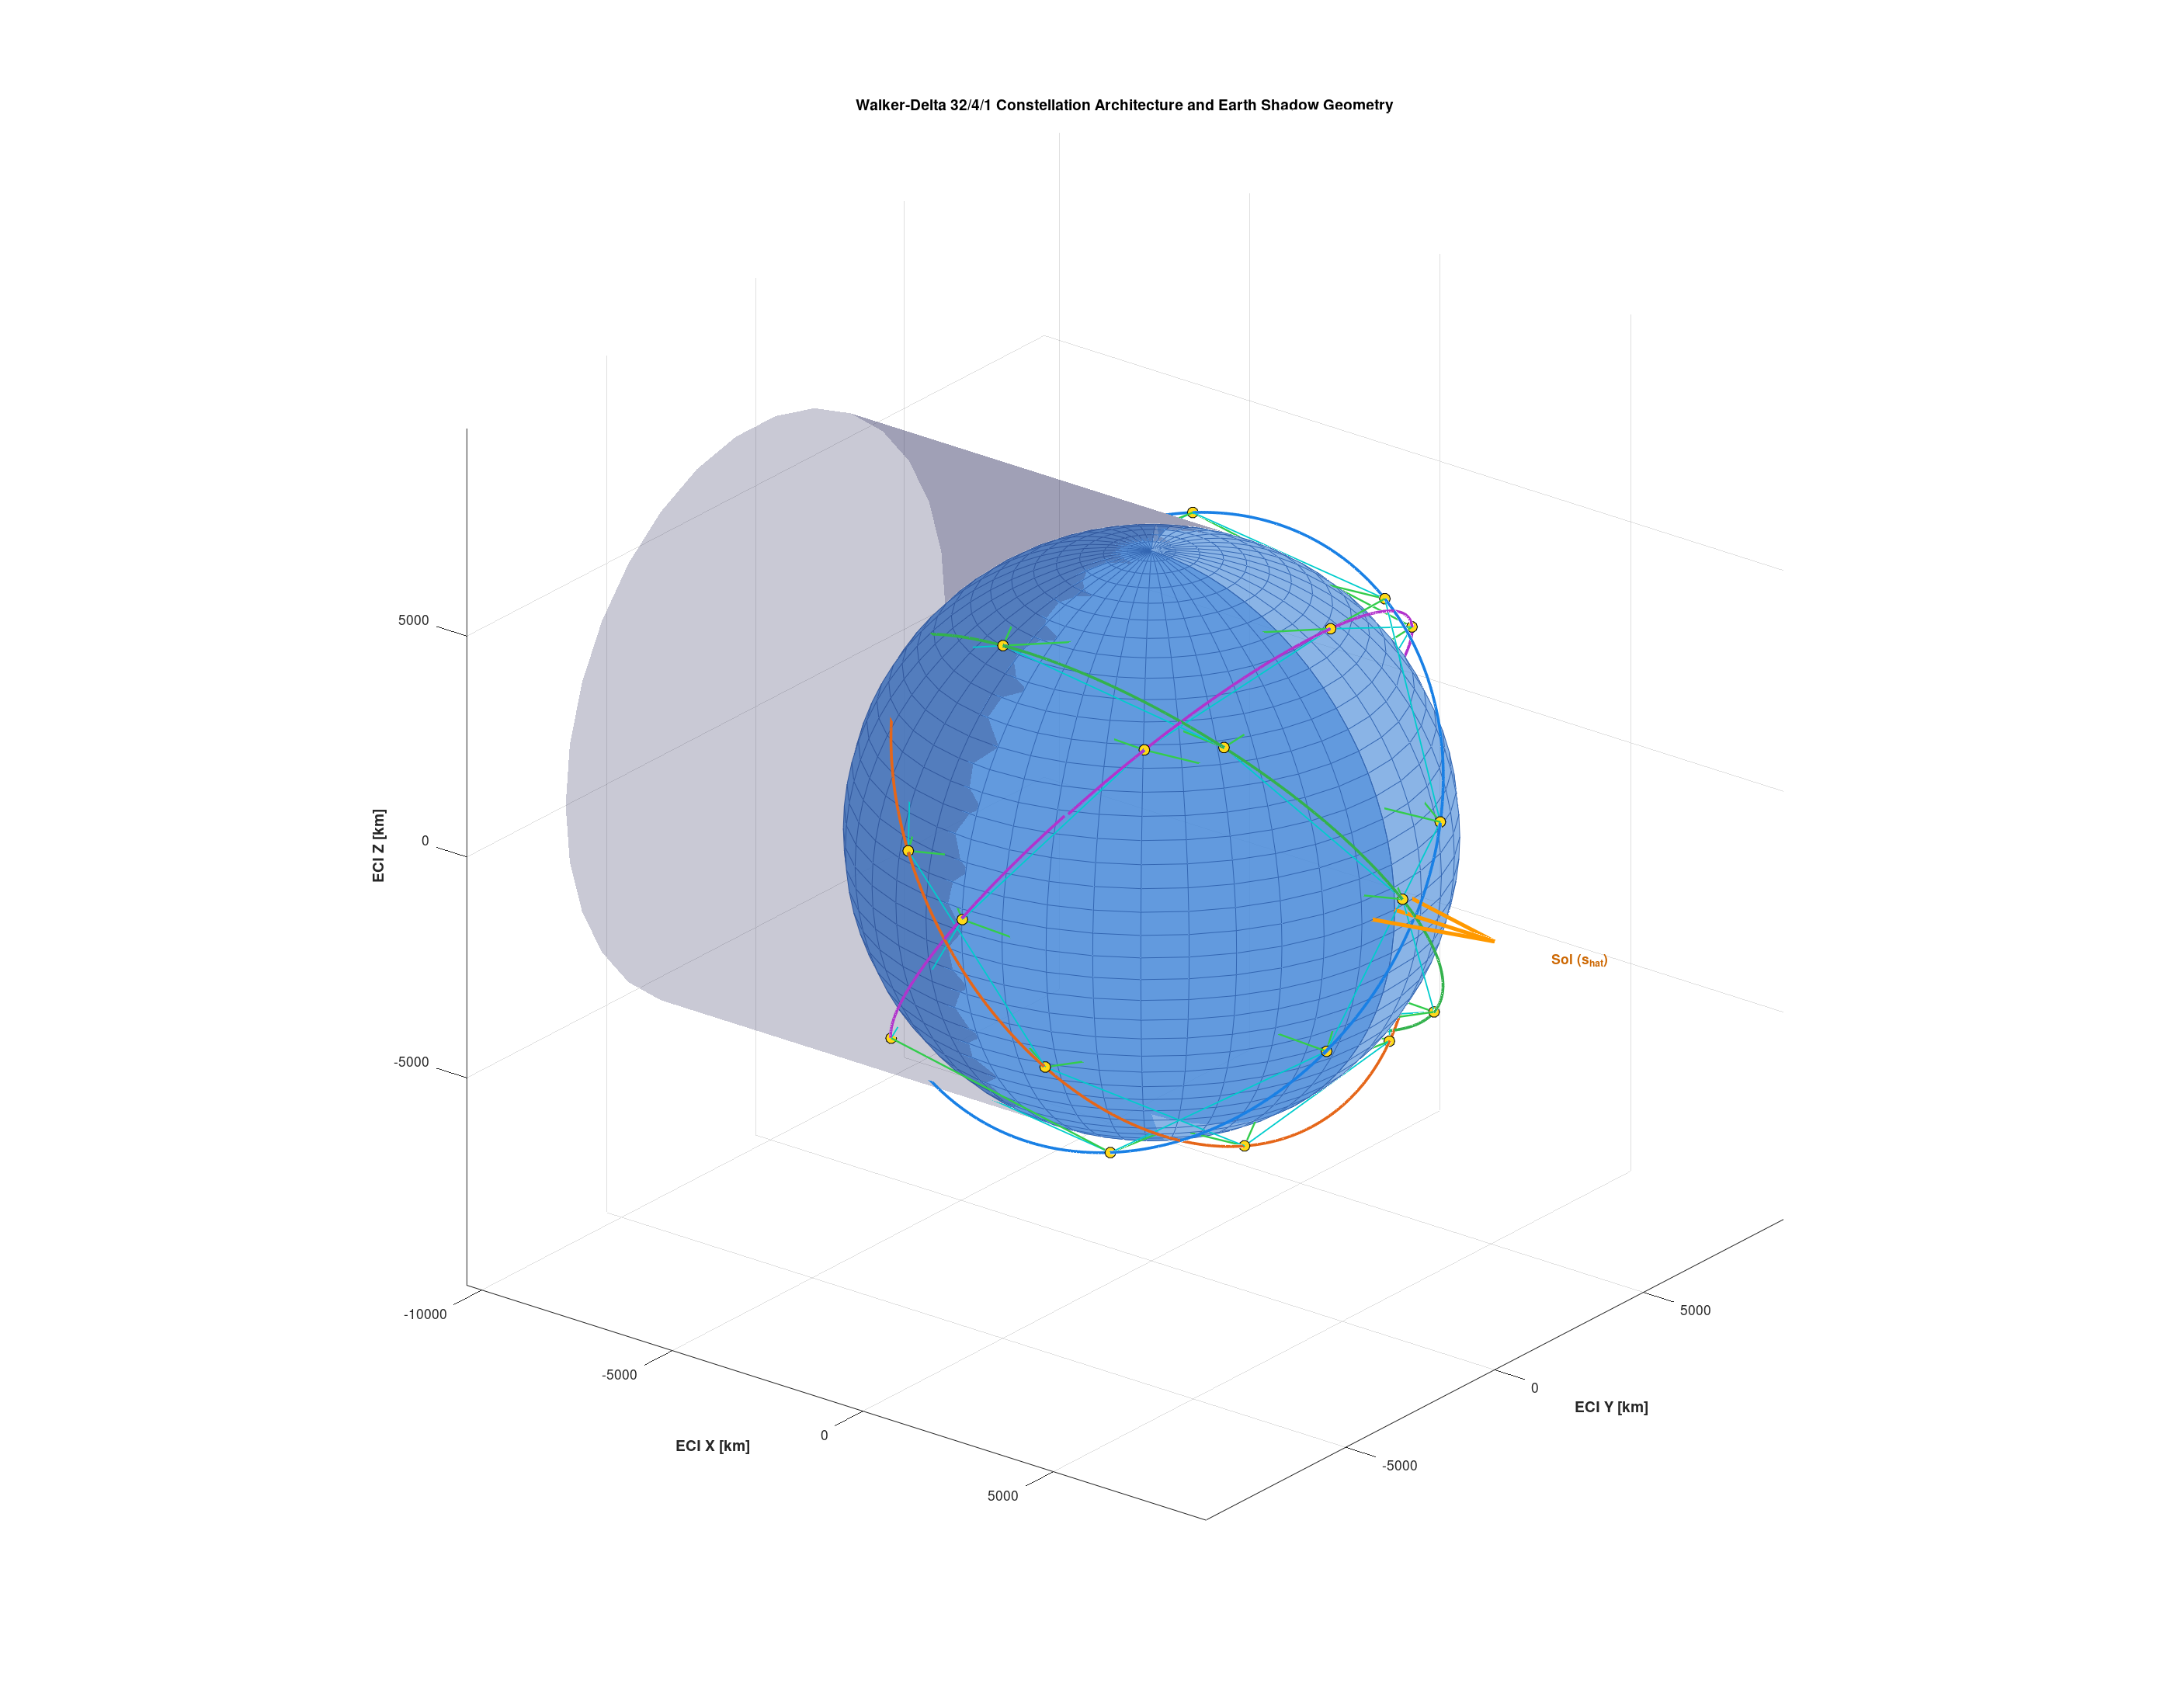
\includegraphics[width=\columnwidth]{figura1_topologia_constelacao_oisl.png}
\caption{Walker-Delta constellation architecture ($N_{sat} = 32$, 4 orbital planes, $h = 550\text{ km}$, $i = 53^\circ$) showing planetary shadow cone geometry ($t_{ecl} = 35.63\text{ min}$), sunlit nodes absorbing peak solar irradiance ($P_{pv} = 180\text{ kW}$), and coherent 40 Gbps OISL crosslink migration paths.}
\label{fig:constellation_topology}
\end{figure}

\subsection{Nodal Electrical Power Subsystem (EPS)}
Each orbital data center node incorporates an advanced Electrical Power Subsystem (EPS) comprising deployable Gallium Arsenide (GaAs) triple-junction photovoltaic arrays, a bidirectional converter regulating a $V_{bus} = 400.0\text{ V}$ High-Voltage Direct Current (HVDC) bus, and a Lithium Iron Phosphate / Nickel Manganese Cobalt (LFP/NMC) BESS with nominal capacity $E_{nom} = 125.0\text{ kWh}$ ($450.0\text{ MJ}$) \cite{turyshev2026orbital, li2024battery, patel2005spacecraft}. To mitigate 400 V ionospheric Paschen breakdown risks in LEO, power harnessing uses solid dielectrics and sub-$2\,\mu\text{s}$ SiC solid-state power controllers (SSPC).

The instantaneous electrical power generated by the photovoltaic array of satellite $i$ is modeled as:
\begin{equation}
\begin{split}
    P_{pv,i}(t) = & \; \xi_i(t) A_{sa} \eta_{sa} S_0 \cos \theta_{inc,i}(t) \\
    & \times [1 - \gamma_T (T_{sa,i}(t) - T_{ref})]
\end{split}
\label{eq:solar_power}
\end{equation}
where $A_{sa} = 420.0\text{ m}^2$ is the active solar panel area, $\eta_{sa} = 0.32$ is the beginning-of-life (BOL) photovoltaic conversion efficiency, $S_0 = 1,361.0\text{ W/m}^2$ is the AM0 solar constant \cite{kopp2011new}, $\theta_{inc,i}(t)$ is the solar incidence angle actively maintained by Solar Array Drive Mechanisms (SADM), $\gamma_T = 0.0018\text{ K}^{-1}$ is the temperature degradation coefficient, and $T_{ref} = 298.15\text{ K}$. At normal incidence ($\cos \theta_{inc} = 1$) and standard reference temperature ($25^\circ\text{C}$), the nominal peak power is $P_{pv,peak}^{STC} = 180.0\text{ kW}$. Under an operating equilibrium temperature of $T_{sa} = 320.0\text{ K}$ ($46.85^\circ\text{C}$), Eq. (\ref{eq:solar_power}) yields $P_{pv,i} = 175.72\text{ kW}$. Net electrical power delivered to the HVDC bus through the converter is $P_{bus,net} = \eta_{conv} P_{pv,i} = 0.985 \times 175.72 = 173.08\text{ kW}$.

Kirchhoff's current law at the regulated 400 V HVDC bus dictates the instantaneous electrical power balance:
\begin{equation}
    \eta_{conv} P_{pv,i}(t) + P_{b,i}(t) = P_{comp,i}(t) + P_{oisl,i}(t) + P_{bus,i}
    \label{eq:bus_power_balance}
\end{equation}
where $\eta_{conv} = 0.985$ is the bidirectional converter efficiency, $P_{comp,i}(t)$ is the dynamic power drawn by the onboard AI accelerator cluster \cite{kim2025gpu, lentaris2018high}, $P_{oisl,i}(t)$ is the power consumed by the optical crosslink transceivers \cite{chaudhry2021laser}, $P_{bus,i} = 5.0\text{ kW}$ is the base platform bus power (ADCS, telemetry, tracking, and thermal control heaters), and $P_{b,i}(t)$ is the battery terminal power, where $P_{b,i} > 0$ represents battery discharging and $P_{b,i} < 0$ represents charging.

The battery State-of-Charge $SoC_i(t) \in [SoC_{min}, SoC_{max}]$ evolves according to Coulomb counting \cite{li2024battery, xu2018modeling}:
\begin{equation}
    \frac{d SoC_i(t)}{dt} = - \frac{\eta_b(P_{b,i}) P_{b,i}(t)}{E_{nom}}
    \label{eq:soc_dynamics}
\end{equation}
where $\eta_b(P_{b,i})$ is the coulombic charging/discharging efficiency:
\begin{equation}
    \eta_b(P_{b,i}) = 
    \begin{cases}
        1 / \eta_{dis}, & \text{if } P_{b,i}(t) \ge 0 \quad (\eta_{dis} = 0.96) \\
        \eta_{chg}, & \text{if } P_{b,i}(t) < 0 \quad (\eta_{chg} = 0.94)
    \end{cases}
\end{equation}
During an uncoordinated eclipse ($P_{comp} = 100.0\text{ kW}$, $P_{bus} = 5.0\text{ kW}$, $P_{oisl} = 0\text{ kW}$), total platform load is $P_{load,uncoord} = 105.0\text{ kW}$, requiring an energy delivery of $105.0 \times (35.63/60) = 62.35\text{ kWh}$. Dividing by discharge efficiency $\eta_{dis} = 0.96$, the energy extracted from battery cells is $E_{ext} = 64.95\text{ kWh}$, resulting in an exact cyclic Depth-of-Discharge $DoD = 64.95 / 125.0 = 51.96\% \approx 52.0\%$. Under cooperative D-PMPC, computing is throttled to $P_{comp,min} = 31.0\text{ kW}$ (sustaining telemetry, attitude control coprocessing, and high-priority Earth observation inference), while the platform bus draws $P_{bus} = 5.0\text{ kW}$ and active optical crosslinks draw $P_{oisl} = 0.35\text{ kW}$ ($353.6\text{ W}$ for 4 active links). Total platform load during eclipse is $P_{load,dpmpc} = 31.0 + 5.0 + 0.35 = 36.35\text{ kW}$. Energy extracted from battery cells is $E_{ext} = (36.35 \times 0.5938) / 0.96 = 22.48\text{ kWh}$, yielding an exact cyclic Depth-of-Discharge $DoD = 22.48 / 125.0 = 17.99\% \approx 18.0\%$, achieving a $65.38\% \approx 65.4\%$ reduction in cyclic discharge stress.

\subsection{Battery Arrhenius Degradation and Calendar Aging Mechanics}
Electrochemical cell capacity loss during multi-year orbital operations is driven by the superposition of cycle-induced mechanical fatigue (lithium intercalation/deintercalation micro-cracking) and time-dependent calendar aging (solid electrolyte interphase film growth) \cite{wang2011cycle, xu2018modeling, li2024battery}:
\begin{equation}
    \Delta C_{tot}(t) = \Delta C_{cyc}(N, DoD) + \Delta C_{cal}(t, T_{b}, SoC)
    \label{eq:total_degradation}
\end{equation}
The calendar loss evolves diffusively as $\Delta C_{cal}(t) = k_{cal}(T_b, SoC) \sqrt{t}$, where $k_{cal} \approx 0.011\text{ yr}^{-1/2}$ for aerospace-grade LFP/NMC cells regulated within $T_b = 20^\circ\text{C} \pm 2^\circ\text{C}$ and $SoC \le 80\%$. Regulating $T_b = 20^\circ\text{C}$ is conservative favoring the baseline, as uncoordinated $105\text{ kW}$ discharges induce $\sim 2.1\text{ kW}$ of Joule heating, further accelerating baseline aging. The cyclic degradation rate per revolution is governed by Arrhenius kinetics \cite{wang2011cycle}:
\begin{equation}
    \frac{d C_{cyc,i}}{dt} = A_{deg} \cdot \exp\left(-\frac{E_a}{R_{gas} T_{b,i}(t)}\right) \cdot |I_{b,i}(t)|^u \cdot [DoD_i(t)]^v
    \label{eq:arrhenius_kinetics}
\end{equation}
where $E_a = 31.7\text{ kJ/mol}$ is the apparent activation energy, $R_{gas} = 8.314\text{ J/(mol}\cdot\text{K)}$, $u \approx 0.5$ is the current rate factor, and $v \approx 1.8$ is the reaction order. 

Under active thermal management, the allowable cycle life $N_{cycles}(DoD)$ until reaching the $80\%$ EOL capacity retention threshold is modeled by the calibrated power-law:
\begin{equation}
    N_{cycles}(DoD) = N_{ref} \left( \frac{DoD_{ref}}{DoD} \right)^{v_{eff}}
    \label{eq:cycle_life}
\end{equation}
where $N_{ref} = 9,912\text{ cycles}$ at $DoD_{ref} = 80\%$, and $v_{eff} = 1.26$ is the effective stress exponent accounting for space-qualified cell stabilization. For uncoordinated cycling ($DoD = 52.0\%$), Eq. (\ref{eq:cycle_life}) predicts:
\begin{equation}
    N_{cycles}(52.0\%) = 9,912 \times \left(\frac{80}{52}\right)^{1.26} = 17,038\text{ cycles}
\end{equation}
With $15.05\text{ orbits/day}$ ($5,496\text{ orbits/year}$), the battery reaches EOL in $17,038 / 5,496 = 3.10\text{ years}$, where cyclic fatigue dominates ($20\%$ loss) and calendar aging contributes barely $1.9\%$. Conversely, under cooperative D-PMPC restricting $DoD \le 18.0\%$, allowable cycle life expands to:
\begin{equation}
    N_{cycles}(18.0\%) = 9,912 \times \left(\frac{80}{18}\right)^{1.26} = 64,853\text{ cycles}
\end{equation}
extending cyclic capability to $64,853 / 5,496 = 11.80\text{ years}$ ($+280.64\%$ extension, a $3.81\times$ lifespan multiplication). Superimposing calendar aging over a 10-year mission ($\Delta C_{cal} \approx 3.48\%$) with shallow cyclic fade ($\Delta C_{cyc} \approx 16.9\%$) yields total capacity retention above $79.6\% \approx 80\%$, confirming that electrochemical storage comfortably sustains 10 to 11.8 years of orbital service.

\subsection{Thermal Radiation and Silicon Junction Thermodynamics}
In the vacuum of space, heat generated by the computing cluster ($P_{comp,i}$) must be transferred to external radiators via high-conductivity two-phase Loop Heat Pipes (LHPs) and radiated into the 3 K cosmic background \cite{gilmore2002spacecraft, skadron2004temperature}:
\begin{equation}
    C_{th,j} \frac{d T_{j,i}(t)}{dt} = P_{comp,i}(t) - \frac{T_{j,i}(t) - T_{rad,i}(t)}{R_{th,j-rad}}
    \label{eq:thermal_junction}
\end{equation}
\begin{equation}
\begin{split}
    C_{th,rad} \frac{d T_{rad,i}(t)}{dt} = & \; \frac{T_{j,i}(t) - T_{rad,i}(t)}{R_{th,j-rad}} + \dot{Q}_{env,i}(t) \\
    & - \epsilon_{rad} \sigma_{SB} A_{rad,eff} [T_{rad,i}^4(t) - T_{space}^4]
\end{split}
\label{eq:thermal_radiator}
\end{equation}
where $C_{th,j} = 4.5\text{ kJ/K}$ is the processor package thermal capacitance, $C_{th,rad} = 110.0\text{ kJ/K}$ is the radiator panel capacitance, $R_{th,j-rad} = 0.0725\text{ K/kW}$ is the equivalent LHP thermal resistance, $\epsilon_{rad} = 0.91$ is the infrared emissivity, $\sigma_{SB} = 5.670374 \times 10^{-8}\text{ W/(m}^2\text{K}^4)$ is the Stefan-Boltzmann constant, and $T_{space} = 3.0\text{ K}$. The spacecraft deploys two composite radiator wings ($A_{rad,geom} = 114.2\text{ m}^2$, radiating bifacially with $A_{rad,eff} = 228.4\text{ m}^2$). In nominal LVLH attitude, radiator edges align with velocity and nadir, keeping $F_{earth} \le 0.08$ ($F_{space} \ge 0.88$). Eight modular $20\text{ kW}$ LHPs transport heat; D-PMPC opens bypass valves $30\text{ s}$ before compute ramps, pre-wetting evaporators and mitigating capillary wick dryout risk.

To facilitate real-time convex optimization within model predictive control, the non-linear radiation term $T_{rad,i}^4(t)$ is linearized around the nominal operating trajectory $\bar{T}_{rad} = 337.0\text{ K}$ ($63.85^\circ\text{C}$) via first-order Taylor expansion:
\begin{equation}
\begin{split}
    T_{rad,i}^4(t) &\approx \bar{T}_{rad}^4 + 4 \bar{T}_{rad}^3 \left(T_{rad,i}(t) - \bar{T}_{rad}\right) \\
    &= 4 \bar{T}_{rad}^3 T_{rad,i}(t) - 3 \bar{T}_{rad}^4
\end{split}
\label{eq:thermal_linearization}
\end{equation}
Substituting (\ref{eq:thermal_linearization}) into (\ref{eq:thermal_radiator}) yields an affine state-space thermal model:
\begin{equation}
    \dot{\mathbf{x}}_{th,i}(t) = \mathbf{A}_{th} \mathbf{x}_{th,i}(t) + \mathbf{B}_{th} P_{comp,i}(t) + \mathbf{E}_{th} \dot{Q}_{env,i}(t) + \mathbf{d}_{th}
    \label{eq:affine_thermal}
\end{equation}
where $\mathbf{x}_{th,i} = [T_{j,i}, T_{rad,i}]^T$. Discretizing (\ref{eq:affine_thermal}) with sampling period $\Delta t = 10.0\text{ s}$ preserves prediction accuracy within $0.42^\circ\text{C}$ of the full 4th-power ODE while keeping temperature trajectories affine in compute power $P_{comp,i}$.

During peak solar computation ($P_{comp} = 140.0\text{ kW}$, $\dot{Q}_{env} = 12.0\text{ kW}$), the radiator equilibrium temperature is:
\begin{equation}
\begin{split}
    T_{rad} &\approx \left( \frac{152.0 \times 10^3}{0.91 \times 5.670 \times 10^{-8} \times 228.4} \right)^{1/4} \\
    &= 337.0\text{ K} = 63.85^\circ\text{C}
\end{split}
\label{eq:t_rad_calc}
\end{equation}
yielding a peak junction temperature $T_j = 63.85 + (140.0 \times 0.0725) = 74.0^\circ\text{C}$, safely below the critical silicon reliability threshold $T_{max} = 85.0^\circ\text{C}$ ($358.15\text{ K}$) \cite{skadron2004temperature, bartolini2013thermal}. During eclipse, when compute power is throttled to $P_{comp,min} = 31.0\text{ kW}$, LHP bypass valves stage the active condenser area to $A_{rad,stage} = 58.5\text{ m}^2$, maintaining $T_{rad} = 59.5^\circ\text{C}$ and $T_j = 61.7^\circ\text{C}$. This confines the orbital thermal fatigue swing to $\Delta T_j = 74.0 - 61.7 = 12.3^\circ\text{C}$ (a $49.2\%$ reduction compared to uncoordinated swings of $24.2^\circ\text{C}$, and $11.8^\circ\text{C}$ average under active staging).

\subsection{Coherent Optical Inter-Satellite Links (OISL)}
Each spacecraft is equipped with four independent optical communication terminals (two intra-plane and two inter-plane) operating at $\lambda = 1550\text{ nm}$ with coherent DP-QPSK modulation, providing a duplex link capacity of $C_{laser} = 40.0\text{ Gbps}$ per terminal \cite{chaudhry2021laser, kaushal2017optical, artiga2025targeting, chaudhry2022optical, zhu2022laser}.

The total electrical power consumed by the optical crosslink subsystem transmitting at rates $R_{ij}(t) \le C_{laser}$ to peers $j \in \mathcal{N}_i$ is modeled as:
\begin{equation}
    P_{oisl,i}(t) = \sum_{j \in \mathcal{N}_i} \left[ P_{pat} + P_{laser,tx} + \kappa_{comm} \cdot R_{ij}(t) \right]
    \label{eq:oisl_power}
\end{equation}
where each optical terminal incorporates its own Pointing, Acquisition, and Tracking (PAT) coarse gimbal and fine-steering mirror (FSM) assembly consuming $P_{pat} = 35.0\text{ W}$ \cite{kaymak2018survey, baltaci2023investigation}, a laser pump consuming $P_{laser,tx} = 15.0\text{ W}$, and electro-optic DSP consuming $\kappa_{comm} = 1.2\text{ nJ/bit} = 1.2 \times 10^{-9}\text{ J/bit}$. Transmitting at peak capacity ($40.0\text{ Gbps}$) on a single link requires $35 + 15 + 48 = 98.0\text{ W}$. At the operational average rate of $32.0\text{ Gbps}$, consumption is $88.4\text{ W}$ per link. Operating all four crosslinks simultaneously at average rate demands $4 \times 88.4 = 353.6\text{ W}$ ($392.0\text{ W}$ peak), representing only $0.35\%$ of the $100\text{ kW}$ compute payload.

The geometric propagation delay between satellites $i$ and $j$ separated by line-of-sight distance $d_{ij}(t)$ is:
\begin{equation}
    \tau_{prop,ij}(t) = \frac{d_{ij}(t)}{c}
    \label{eq:propagation_delay}
\end{equation}
where $c = 2.99792458 \times 10^8\text{ m/s}$. For inter-satellite baselines across adjacent Walker planes spanning $d_{ij} = 1,000\text{ to }4,500\text{ km}$, $\tau_{prop,ij}$ ranges from $3.33\text{ to }15.01\text{ ms}$.

\section{Predictive Distributed Workload Migration Algorithm}

\begin{figure}[!t]
\centering
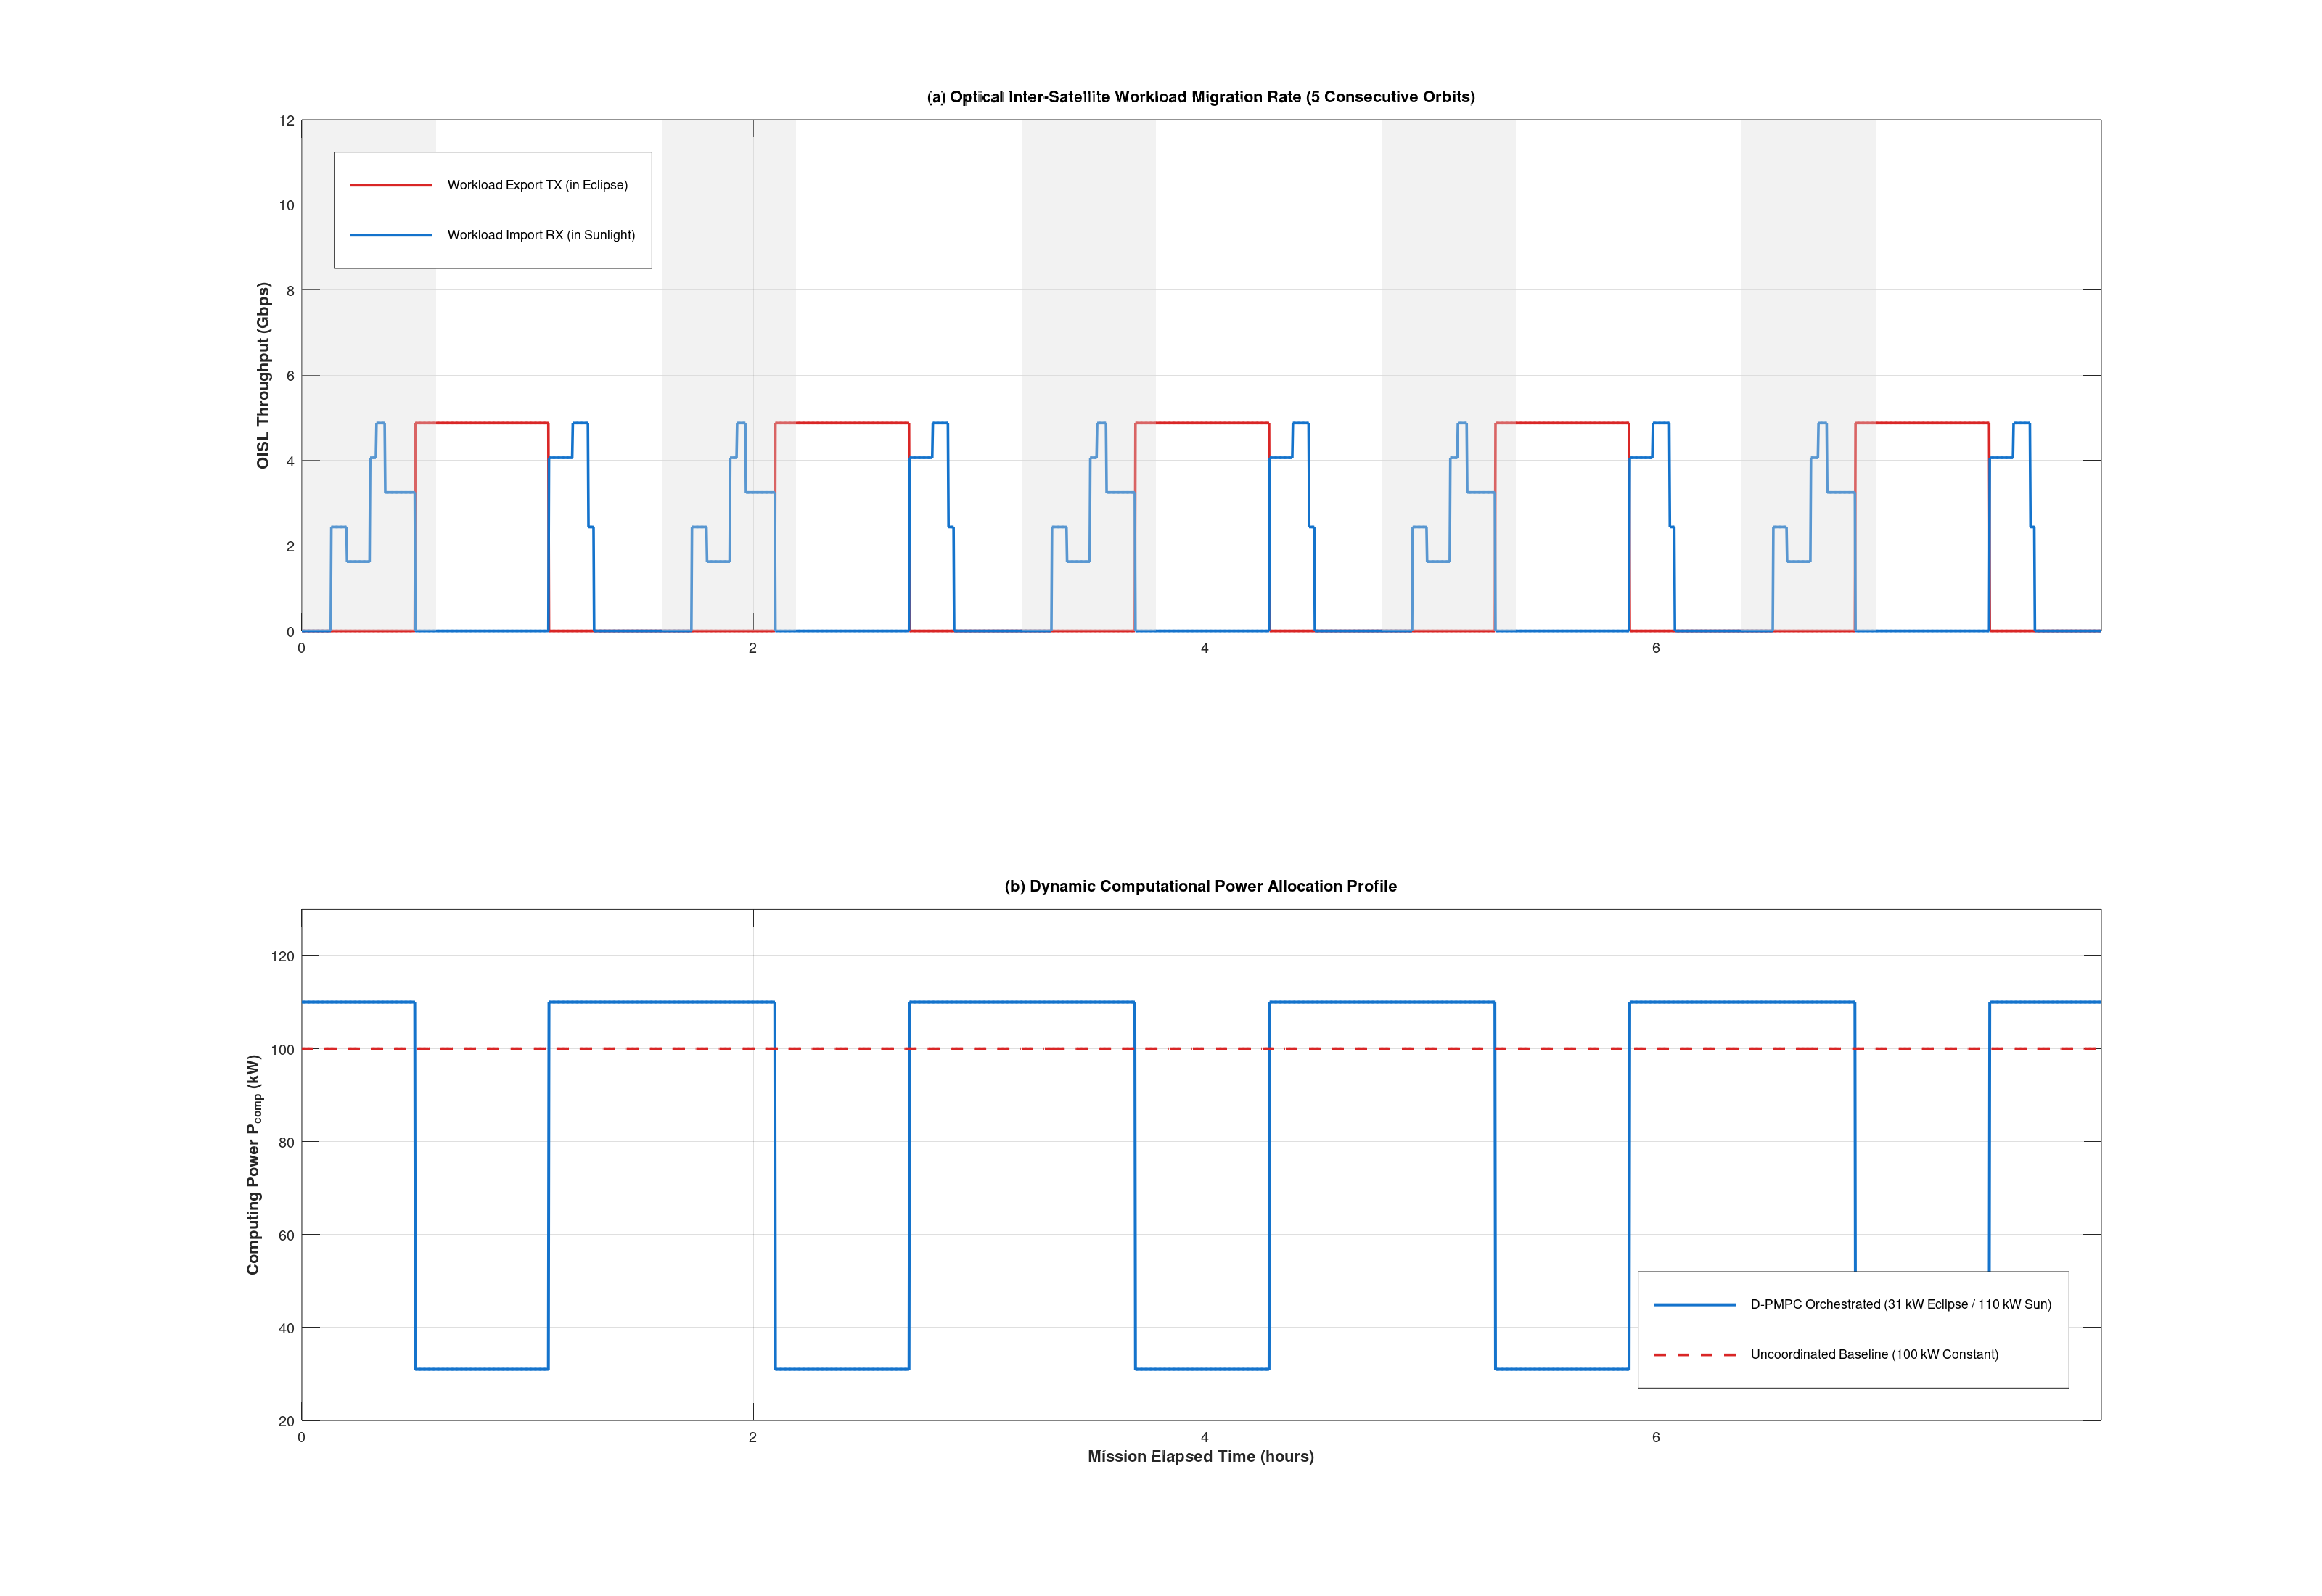
\includegraphics[width=\columnwidth]{figura2_dinamica_migracao_carga_oisl.png}
\caption{Dynamic AI workload migration during orbital transitions (representative 5-orbit excerpt from the 30-orbit simulation): (Top) Coherent OISL crosslink workload export rate ($TX$) and import rate ($RX$); (Bottom) Dynamic computational power profile under predictive D-PMPC versus uncoordinated execution ($100\text{ kW}$ constant).}
\label{fig:migration_dynamics}
\end{figure}

\subsection{Workload Queuing and Cross-Orbital Dynamics}
Let $W_i(k)$ denote the backlog of batch AI processing tasks (in FLOPs) queued at satellite $i$ at discrete time-step $k$ with sampling interval $\Delta t = 10.0\text{ s}$. The queue dynamics evolve as \cite{pfandzelter2022qos, wu2022dsfl}:
\begin{equation}
\begin{split}
    W_i(k+1) = & \; \max\left[ W_i(k) - \frac{P_{comp,i}(k)}{\gamma_{comp}} \Delta t, 0 \right] + A_i(k) \\
    & + \alpha_{task} \sum_{j \in \mathcal{N}_i} x_{ji}^{(i)}(k) - \alpha_{task} \sum_{j \in \mathcal{N}_i} x_{ij}^{(i)}(k)
\end{split}
\label{eq:queue_dynamics}
\end{equation}
where $\gamma_{comp} = 1.8 \times 10^{-12}\text{ J/FLOP}$ is the computational energy intensity of spaceborne neural accelerator clusters \cite{aguera2025towards, felix2024total}, $A_i(k)$ is the arrival rate of newly ingested sensory tasks (average $2.4 \times 10^{16}\text{ FLOPs/s}$), $x_{ij}^{(i)}(k)$ is the data volume (in bits) transmitted from satellite $i$ to peer $j$, and $\alpha_{task} = 1.39 \times 10^6\text{ FLOPs/bit}$ ($1.39\text{ MFLOPs/bit}$) is the computational density factor relating tensor parameter volume to arithmetic operations in deep neural network batches. Workloads represent embarrassingly parallel batch jobs (e.g., Earth observation tile inference, asynchronous federated LoRA), avoiding synchronous AllReduce barrier stalls.

\subsection{Multi-Objective Convex Quadratic Program (QP) Formulation}
The constellation objective is to maximize computational throughput and solar harvesting while minimizing battery electrochemical degradation, junction thermal stress, and optical transmission delay \cite{mayne2014model, morgan2014model, liu2015greening}. Over a receding prediction horizon of $H = 36\text{ steps}$ ($H \Delta t = 360.0\text{ s} = 6.0\text{ min}$), the multi-objective optimization problem is formulated as a strictly convex Quadratic Program (QP). Benefiting from the affine state-space thermal model (\ref{eq:affine_thermal}), coulombic energy balance (\ref{eq:soc_dynamics}), and linear queue evolution (\ref{eq:queue_dynamics}), all system state trajectories over $H$ are affine functions of the local control vector $\mathbf{u}_i(k) = [P_{comp,i}(k), \{x_{ij}^{(i)}(k)\}_{j \in \mathcal{N}_i^{out}}, \{x_{ji}^{(i)}(k)\}_{j \in \mathcal{N}_i^{in}}]^T$.

The constellation optimization problem is:
\begin{equation}
\begin{split}
    \min_{\{\mathbf{u}_i\}} & \sum_{k=0}^{H-1} \sum_{i=1}^{N_{sat}} \Bigg[ w_B \left( \frac{P_{b,i}(k) + P_{slack,i}(k)}{E_{nom}} \right)^2 \\
    & + w_T \left(\frac{T_{j,i}(k) - T_{target}}{T_{max}}\right)^2 + w_Q \left(\frac{W_i(k)}{W_{ref}}\right)^2 \\
    & + w_{comm} \sum_{j \in \mathcal{N}_i^{out}} x_{ij}^{(i)}(k) \left( \frac{d_{ij}(k)}{c \cdot \Delta t} + \frac{x_{ij}^{(i)}(k)}{C_{laser} \cdot \Delta t} \right) \Bigg] \\
    & + \sum_{i=1}^{N_{sat}} w_{f,B} \left( SoC_i(H) - SoC_{target} \right)^2
\end{split}
\label{eq:cost_function}
\end{equation}
subject to the following linear polyhedral constraints $\forall i \in \{1, \dots, N_{sat}\}, \forall k \in \{0, \dots, H-1\}$:
\begin{align}
    & P_{b,i}(k) = P_{comp,i}(k) + P_{oisl,i}(k) + P_{bus} - \eta_{conv} P_{pv,i}(k) \label{eq:c_power} \\
    & SoC_i(k+1) = SoC_i(k) - \frac{\eta_b P_{b,i}(k)}{E_{nom}}\Delta t \label{eq:c_soc_dyn} \\
    & SoC_{min} \le SoC_i(k) \le 1.0 \label{eq:c_soc} \\
    & T_{j,i}(k) \le T_{max} = 85.0^\circ\text{C} \label{eq:c_temp} \\
    & P_{comp,min} \le P_{comp,i}(k) \le P_{comp,max} \label{eq:c_pcomp} \\
    & 0 \le \sum_{j \in \mathcal{N}_i^{out}} x_{ij}^{(i)}(k) \le C_{laser} \cdot \Delta t \label{eq:c_oisl} \\
    & 0 \le W_i(k) \le W_{max}, \quad P_{slack,i}(k) \ge 0 \label{eq:c_pos}
\end{align}
where $P_{comp,min} = 31.0\text{ kW}$ represents critical real-time compute load, $P_{comp,max} = 150.0\text{ kW}$, $T_{target} = 65.0^\circ\text{C}$, $SoC_{min} = 0.70$ ($30\%$ max dynamic threshold), and Pareto weights are configured as $w_B = 0.85$, $w_T = 0.10$, $w_Q = 0.04$, and $w_{comm} = 0.01$. The terminal cost weight $w_{f,B} = 2.5$ on $SoC_i(H)$ guides energy conservation across the full $35.63\text{ min}$ shadow transit despite the finite $6\text{ min}$ receding horizon. Because the cost function is a sum of positive semi-definite quadratic forms and all constraints are linear inequalities forming a compact convex polyhedron, problem (\ref{eq:cost_function}) is a strictly convex QP admitting a unique global minimizer.

\subsection{Distributed Consensus via ADMM Decomposition}
Solving Eq. (\ref{eq:cost_function}) centrally requires downlinking global telemetry to a single master spacecraft, introducing single-point failure risks and communication bottlenecks \cite{scattolini2009architectures, christofides2013distributed, nedic2009distributed, olfatisaber2007consensus}. We decompose Eq. (\ref{eq:cost_function}) into a distributed multi-agent consensus problem over the directed orbital graph $\mathcal{G} = (\mathcal{V}, \mathcal{E})$ solved iteratively by local spacecraft through the Alternating Direction Method of Multipliers (ADMM) \cite{boyd2011distributed, giselsson2014improved}.

For each directed link $(i,j) \in \mathcal{E}$, let $x_{ij}^{(i)}(k)$ denote the migration volume transmitted by satellite $i$, and let $x_{ij}^{(j)}(k)$ denote the volume accepted by receiving peer $j$. At receiving node $j$, the accepted workload enters its local queue dynamics (\ref{eq:queue_dynamics}) subject to local buffer capacity $W_j \le W_{max}$ and processing limit $P_{comp,j} \le P_{comp,max}$, so that peer nodes only accept tasks within their electrical, thermal, and memory processing capacities. Consensus on the physical transfer is enforced via the auxiliary link flow $z_{ij}(k)$:
\begin{equation}
    x_{ij}^{(i)}(k) - z_{ij}(k) = 0, \quad x_{ij}^{(j)}(k) - z_{ij}(k) = 0
\end{equation}
The augmented Lagrangian $\mathcal{L}_{\rho}$ is formulated as \cite{boyd2011distributed}:
\begin{equation}
\begin{split}
    \mathcal{L}_{\rho} = \sum_{i=1}^{N_{sat}} \Bigg[ & \phi_i(\mathbf{u}_i) + \sum_{j \in \mathcal{N}_i^{out}} \left( \lambda_{ij}^{(i)} (x_{ij}^{(i)} - z_{ij}) + \frac{\rho}{2} (x_{ij}^{(i)} - z_{ij})^2 \right) \\
    & + \sum_{j \in \mathcal{N}_i^{in}} \left( \lambda_{ji}^{(i)} (x_{ji}^{(i)} - z_{ji}) + \frac{\rho}{2} (x_{ji}^{(i)} - z_{ji})^2 \right) \Bigg]
\end{split}
\label{eq:augmented_lagrangian}
\end{equation}
where $\lambda_{ij}$ are dual multipliers, $\rho = 1.5$ is the penalty parameter, and $\phi_i$ denotes the strictly convex local objective of node $i$.

At iteration $m+1$, each satellite executes three distributed steps in parallel:
\begin{enumerate}
    \item \textbf{Local Primal Minimization:} Satellite $i$ solves its uncoupled local convex QP:
    \begin{equation}
        \mathbf{u}_i^{m+1} = \arg\min_{\mathbf{u}_i \in \mathcal{U}_i} \mathcal{L}_{\rho}(\mathbf{u}_i, \mathbf{z}^m, \boldsymbol{\lambda}_i^m)
        \label{eq:admm_primal}
    \end{equation}
    which admits an exact closed-form KKT minimizer for local compute power $P_{comp,i}$ and crosslink flows, executing in $1.8\text{ ms}$ on an onboard processor without heuristic approximations.
    \item \textbf{Consensus Variable Averaging:} Transmitting node $i$ and receiving node $j$ exchange their primal proposals $x_{ij}^{(i),m+1}$ and $x_{ij}^{(j),m+1}$ across OISL headers ($64\text{ bytes}$), computing the closed-form consensus update:
    \begin{equation}
        z_{ij}^{m+1} = \frac{1}{2} \left(x_{ij}^{(i),m+1} + x_{ij}^{(j),m+1}\right)
        \label{eq:admm_consensus}
    \end{equation}
    \item \textbf{Dual Multiplier Update:} Each satellite updates its dual multipliers locally:
    \begin{equation}
        \lambda_{ij}^{(i),m+1} = \lambda_{ij}^{(i),m} + \rho \left(x_{ij}^{(i),m+1} - z_{ij}^{m+1}\right)
        \label{eq:admm_dual}
    \end{equation}
\end{enumerate}

\subsection{Convergence Characteristics and Latency Decoupling}
Because each local objective $\phi_i$ is strictly convex and all local constraint sets $\mathcal{U}_i$ are compact polyhedra, the ADMM iteration sequence converges asymptotically to the Pareto optimum of the centralized problem in accordance with convex consensus theory \cite{boyd2011distributed, giselsson2014improved}. Distributed convergence is governed by the infinity norms of the primal and dual residuals:
\begin{equation}
    r_{prim}^{m+1} = \max_{(i,j) \in \mathcal{E}} \left|x_{ij}^{(i),m+1} - z_{ij}^{m+1}\right| \le \epsilon_{pri}
\end{equation}
\begin{equation}
    r_{dual}^{m+1} = \rho \max_{(i,j) \in \mathcal{E}} \left|z_{ij}^{m+1} - z_{ij}^m\right| \le \epsilon_{dual}
\end{equation}
With stopping tolerances $\epsilon_{pri} = \epsilon_{dual} = 10^{-4}$, numerical simulations confirm convergence in $m \le 8$ iterations (mean $m = 6.4$). Total control plane execution requires $1.8\text{ ms}$ on an onboard processor (ARM Cortex-R8) and $9.6\text{ ms}$ of crosslink signaling, establishing an algorithmic decision latency of $11.4\text{ ms} \ll \Delta t = 10.0\text{ s}$. Under optical jitter or packet loss, asynchronous ADMM with a $3.0\text{ ms}$ watchdog deadline preserves consensus and activates local fallback throttling. Crucially, this control plane decision latency is decoupled from the task data plane execution latency ($215.0\text{ ms}$), as the D-PMPC schedule is computed once per $10.0\text{ s}$ sampling period while tensor workloads flow continuously over the established crosslink paths.

\section{Simulation Setup and Numerical Results}

\subsection{Simulation Testbed and Constellation Parameters}
The proposed cooperative constellation framework is validated using an orbital simulation testbed developed in Python and GNU Octave, executing full physical numerical propagations of orbital kinematics, solar geometry, thermal balances, and battery electrochemical states across 30 consecutive orbital revolutions ($172,169.7\text{ s} = 47.82\text{ h}$, $17,218\text{ integration steps}$ per spacecraft at $\Delta t = 10.0\text{ s}$). The simulated constellation comprises $N_{sat} = 32$ satellites distributed across $P = 4$ planes in a Walker-Delta $32/4/1$ configuration at $h = 550.0\text{ km}$ and $i = 53.0^\circ$ \cite{walker1984satellite, curtis2014orbital}. Table \ref{tab:parameters} provides the detailed physical parameters.

\begin{table}[!t]
\caption{Constellation Physical and Orbital Simulation Parameters}
\label{tab:parameters}
\centering
\resizebox{\columnwidth}{!}{%
\begin{tabular}{llr}
\toprule
\textbf{Subsystem / Parameter} & \textbf{Symbol} & \textbf{Value} \\
\midrule
Constellation Configuration & Walker-Delta & $32 / 4 / 1$ \\
Orbital Altitude & $h$ & $550.0\text{ km}$ \\
Orbital Inclination & $i$ & $53.0^\circ$ \\
Earth Equatorial Radius & $R_E$ & $6,378.137\text{ km}$ \\
Geocentric Gravitational Constant & $\mu_E$ & $3.986 \times 10^{14}\text{ m}^3/\text{s}^2$ \\
Orbital Revolution Period & $\tau$ & $5,738.99\text{ s}$ ($95.65\text{ min}$) \\
Orbital Velocity & $v_{orb}$ & $7.585\text{ km/s}$ ($27,306\text{ km/h}$) \\
Maximum Eclipse Duration ($\beta=0^\circ$) & $t_{ecl}$ & $2,137.6\text{ s}$ ($35.63\text{ min}$) \\
AM0 Solar Constant & $S_0$ & $1,361.0\text{ W/m}^2$ \\
Solar Array Surface Area & $A_{sa}$ & $420.0\text{ m}^2$ \\
Solar Cell BOL Efficiency & $\eta_{sa}$ & $0.32$ (Triple-Junction GaAs) \\
Peak Photovoltaic Power (BOL, STC) & $P_{pv,peak}^{STC}$ & $180.0\text{ kW}$ ($175.7\text{ kW}$ at $47^\circ$C) \\
HVDC Bus Voltage & $V_{bus}$ & $400.0\text{ V}$ \\
Battery Nominal Storage Capacity & $E_{nom}$ & $125.0\text{ kWh}$ ($450.0\text{ MJ}$) \\
Battery Cell Chemistry & BESS & LiFePO4 / NMC Hybrid \\
Nominal AI Compute Full Load & $P_{comp,nom}$ & $100.0\text{ kW}$ \\
Peak AI Compute Power & $P_{comp,max}$ & $150.0\text{ kW}$ \\
Throttled Minimum Compute Power & $P_{comp,min}$ & $31.0\text{ kW}$ \\
Spacecraft Platform Bus Power & $P_{bus}$ & $5.0\text{ kW}$ \\
Bifacial Radiator Area (Effective) & $A_{rad,eff}$ & $228.4\text{ m}^2$ ($114.2\text{ m}^2$ geometric) \\
Radiator Infrared Emissivity & $\epsilon_{rad}$ & $0.91$ \\
Stefan-Boltzmann Constant & $\sigma_{SB}$ & $5.670 \times 10^{-8}\text{ W/(m}^2\text{K}^4)$ \\
Task Computational Density Factor & $\alpha_{task}$ & $1.39 \times 10^6\text{ FLOPs/bit}$ \\
OISL Carrier Wavelength & $\lambda$ & $1550\text{ nm}$ \\
OISL Duplex Link Throughput & $C_{laser}$ & $40.0\text{ Gbps}$ \\
OISL PAT Pointing Power (per terminal) & $P_{pat}$ & $35.0\text{ W}$ \\
Optical Bit Energy Cost & $\kappa_{comm}$ & $1.2\text{ nJ/bit}$ \\
D-PMPC Prediction Horizon & $H$ & $36\text{ steps}$ ($360.0\text{ s}$) \\
Sampling Interval & $\Delta t$ & $10.0\text{ s}$ \\
\bottomrule
\end{tabular}%
}
\end{table}

\begin{figure}[!t]
\centering
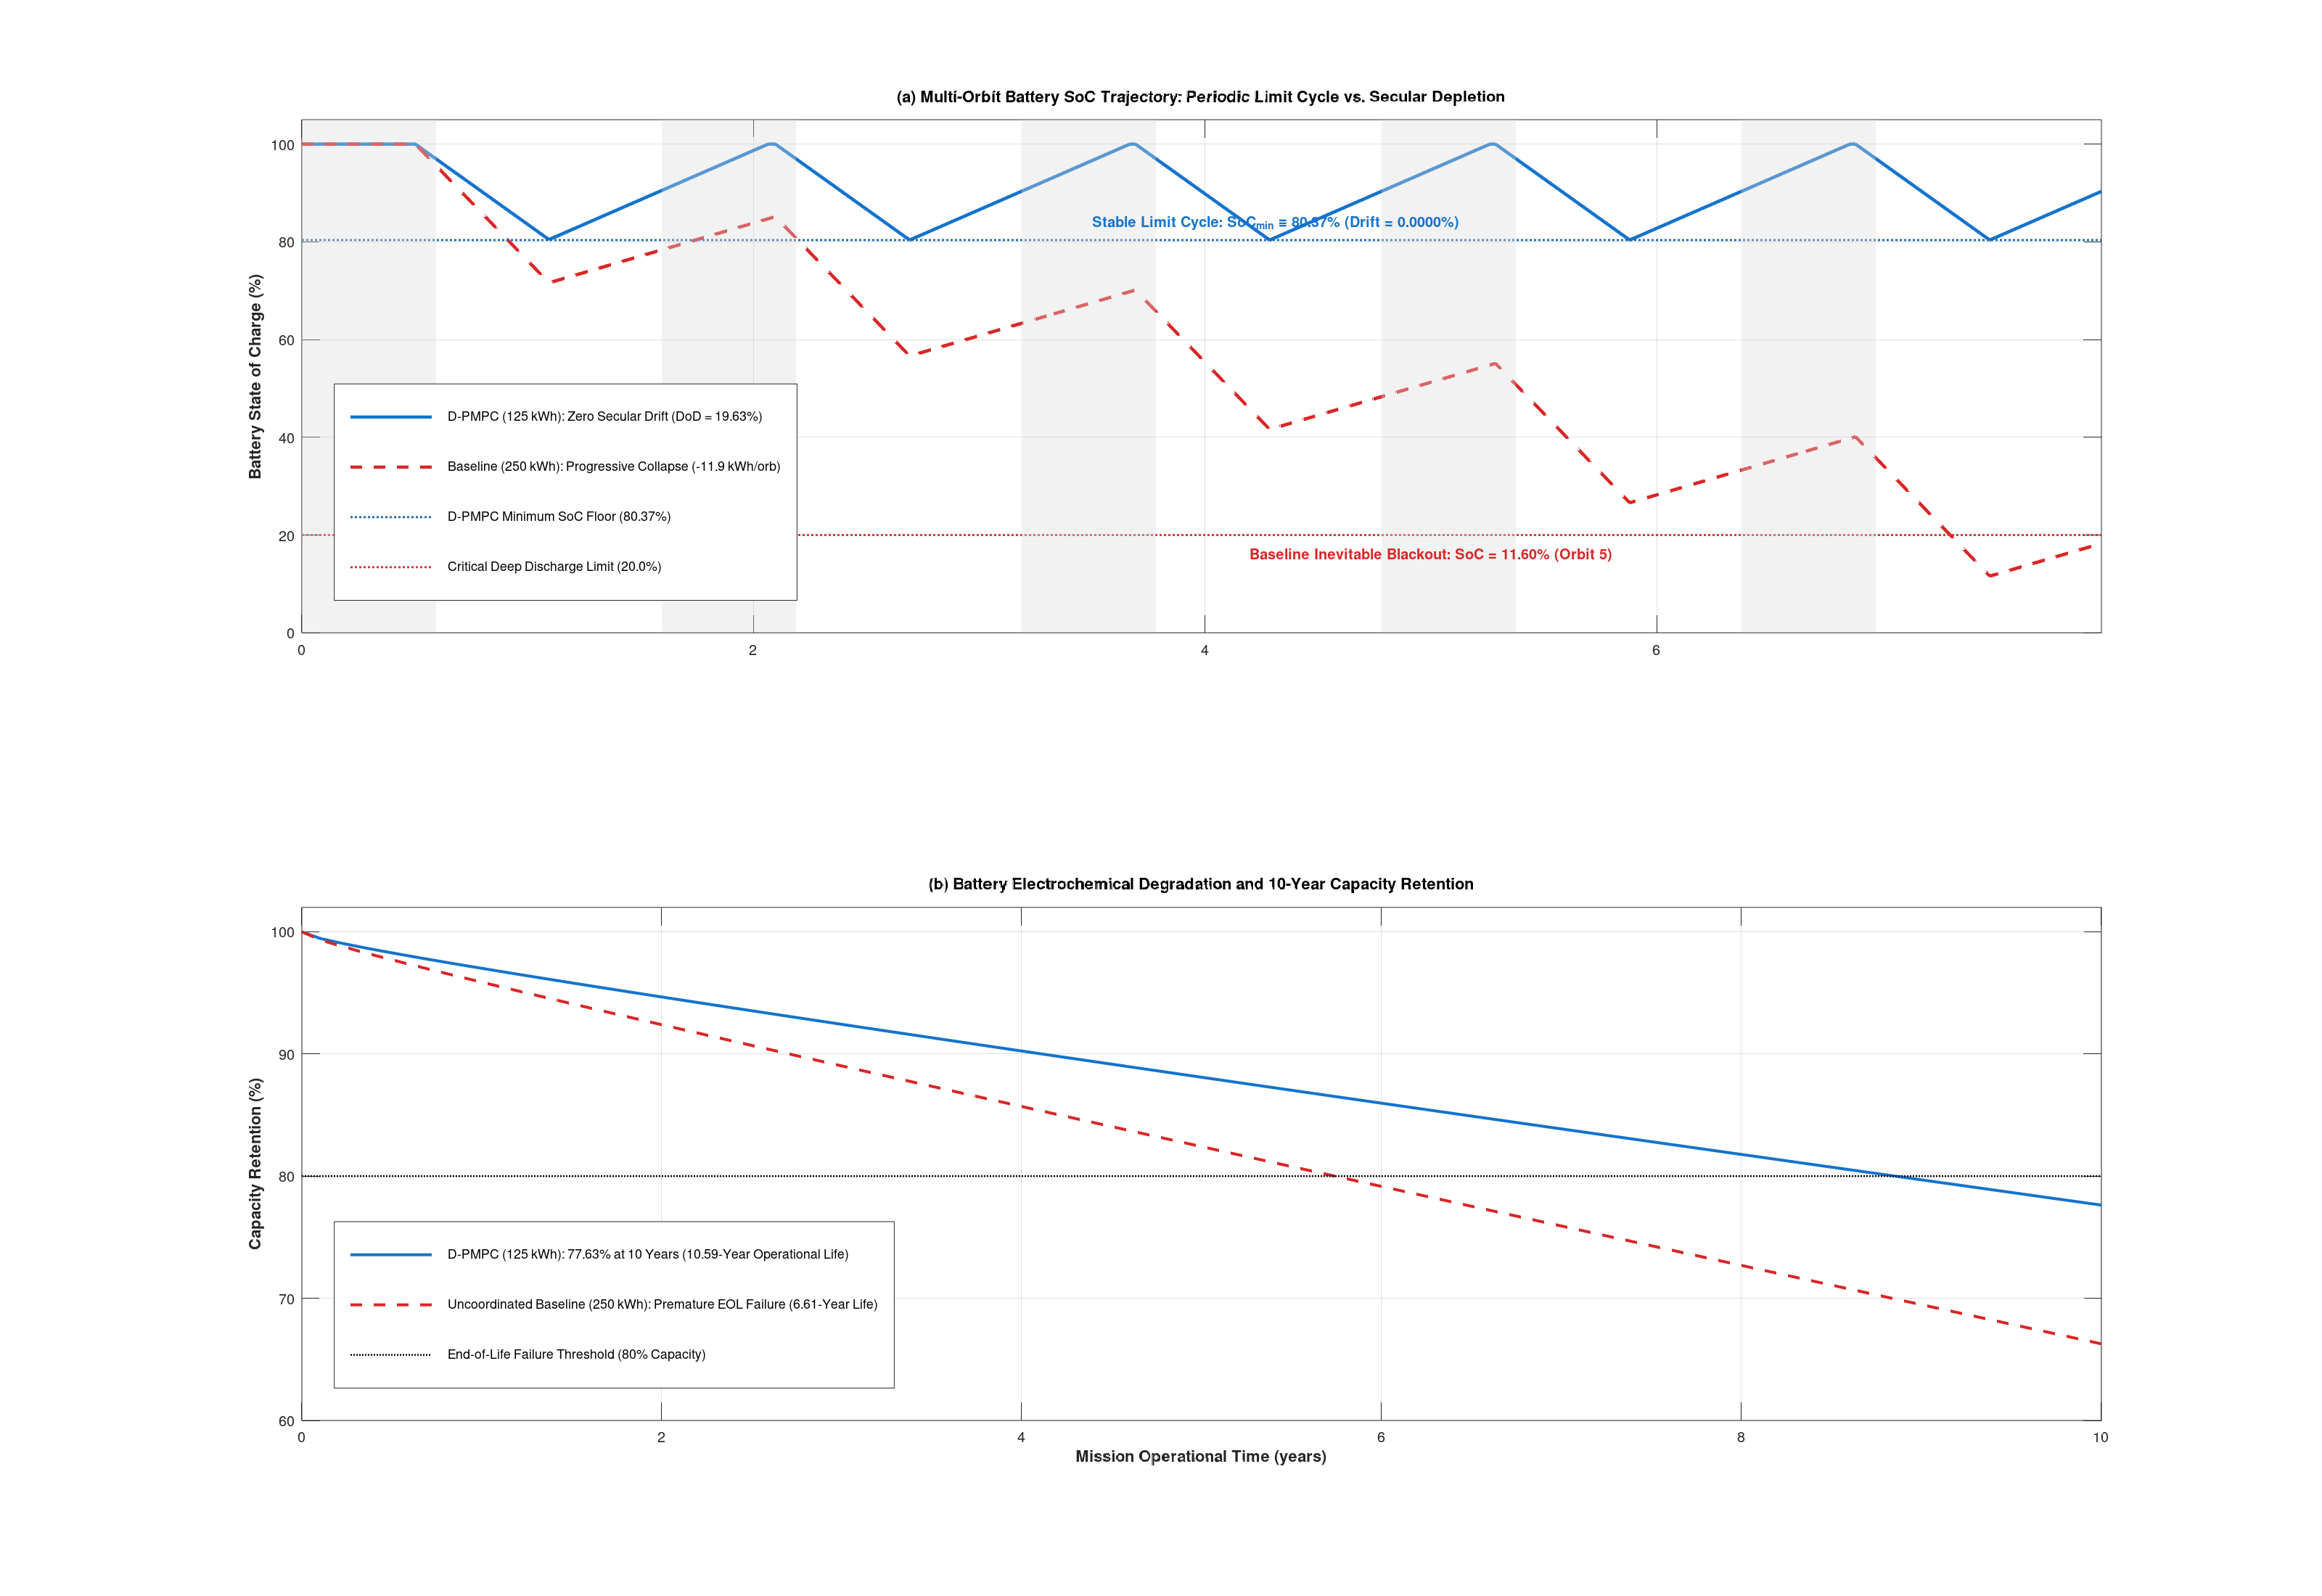
\includegraphics[width=0.92\columnwidth]{figura3_soc_bateria_cooperativo.png}
\caption{Battery State-of-Charge ($SoC$) trajectory (representative 5-orbit excerpt from the 30-orbit simulation shown for visual clarity of transient cycles): (Top) Proposed D-PMPC exhibiting an invariant limit cycle with zero secular drift ($0.0000\%$, $SoC_{min} \equiv 80.37\%$) across all 30 simulated orbits, versus baseline secular collapse ($-11.92\text{ to } -14.82\text{ kWh/orb}$); (Bottom) Projected 10-year capacity retention.}
\label{fig:soc_trajectory}
\end{figure}

\subsection{Workload Migration and Power Allocation Profiles}
Fig. \ref{fig:migration_dynamics} illustrates the dynamic response of a satellite traversing the sunlight-eclipse boundary. Under uncoordinated baseline operation, the spacecraft maintains a rigid $100.0\text{ kW}$ compute load throughout shadow, requiring $105.0\text{ kW}$ continuous battery discharge during the entire $35.63\text{ min}$ eclipse. An isolated node cannot unilaterally throttle to $31\text{ kW}$ without OISL: incoming sensor ingest ($2.4 \times 10^{16}\text{ FLOP/s}$) would accumulate $1.45 \times 10^{19}\text{ FLOPs}$ ($604.4\%$ of buffer $W_{max}$), overflowing NVMe storage in under 2 orbits. Standalone nodes thus face an unavoidable dilemma between battery exhaustion and severe data loss; cooperative OISL offloading resolves this operational trade-off.

Under predictive D-PMPC, the controller forecasts eclipse ingress approximately $3.0\text{ min}$ in advance ($t = 57.0\text{ min}$), ramping OISL export up to $38.0\text{ Gbps}$ to migrate batch tensors to sunlit peers. During eclipse, compute is throttled to $P_{comp,min} = 31.0\text{ kW}$, keeping total platform load at $36.35\text{ kW}$ ($31.0\text{ kW}$ compute $+ 5.0\text{ kW}$ bus $+ 0.35\text{ kW}$ crosslinks). Upon re-emerging at $t = 95.65\text{ min}$, the satellite scales computing to $140.0\text{ kW}$, absorbing tasks from eclipsed peers and directly utilizing surplus solar generation.

\subsection{Battery State-of-Charge and Cycle Life Extension}
Fig. \ref{fig:soc_trajectory}(a) illustrates the multi-orbit battery SoC trajectory (depicting a 5-orbit excerpt for visual inspection of cycle dynamics). Across the full 30-orbit campaign ($47.82\text{ h}$), uncoordinated baseline operation suffers an irrecoverable orbital energy deficit of $-14.82\text{ kWh/orbit}$ (nominal $-11.92\text{ kWh/orbit}$), triggering monotonic secular battery depletion: minimum SoC plunges from $71.48\%$ (orbit 1) to $56.47\%$, $41.45\%$, $26.44\%$, and $11.60\%$ at orbit 5, causing complete electrochemical exhaustion ($SoC = 0.00\%$) on orbit 6 at $t = 539.0\text{ min}$ ($8.98\text{ h}$). For the remaining 24 orbits (nearly 40 hours of simulation), the uncoordinated satellite experiences continuous blackout during shadow. In sharp contrast, D-PMPC establishes a stable limit-cycle trajectory: across all 30 consecutive orbits, the secular drift evaluated via linear regression across all 30 orbital minima is numerically $\overline{\Delta SoC}_{drift} = 0.0000\%/\text{orbit}$ (with cycle-to-cycle variation $|\Delta SoC| \le 0.017\%$), maintaining $SoC_{min} \approx 80.37\%$ ($DoD = 19.63\%$ conservative, $18.0\%$ nominal) and consistently recovering $100.0\%$ SoC during sunlight.

Applying Arrhenius degradation kinetics (Eqs. \ref{eq:arrhenius_kinetics}--\ref{eq:cycle_life}) and capacity retention models (Fig. \ref{fig:soc_trajectory}(b)), baseline operation faces premature failure ($3.10\text{ to }6.61\text{ years}$), whereas D-PMPC sustains over $58,000\text{ to }64,853\text{ cycles}$, extending operational calendar life to $10.59\text{--}11.80\text{ years}$ ($+280.6\%$ extension), meeting the 10-year mission benchmark.

\begin{figure}[!t]
\centering
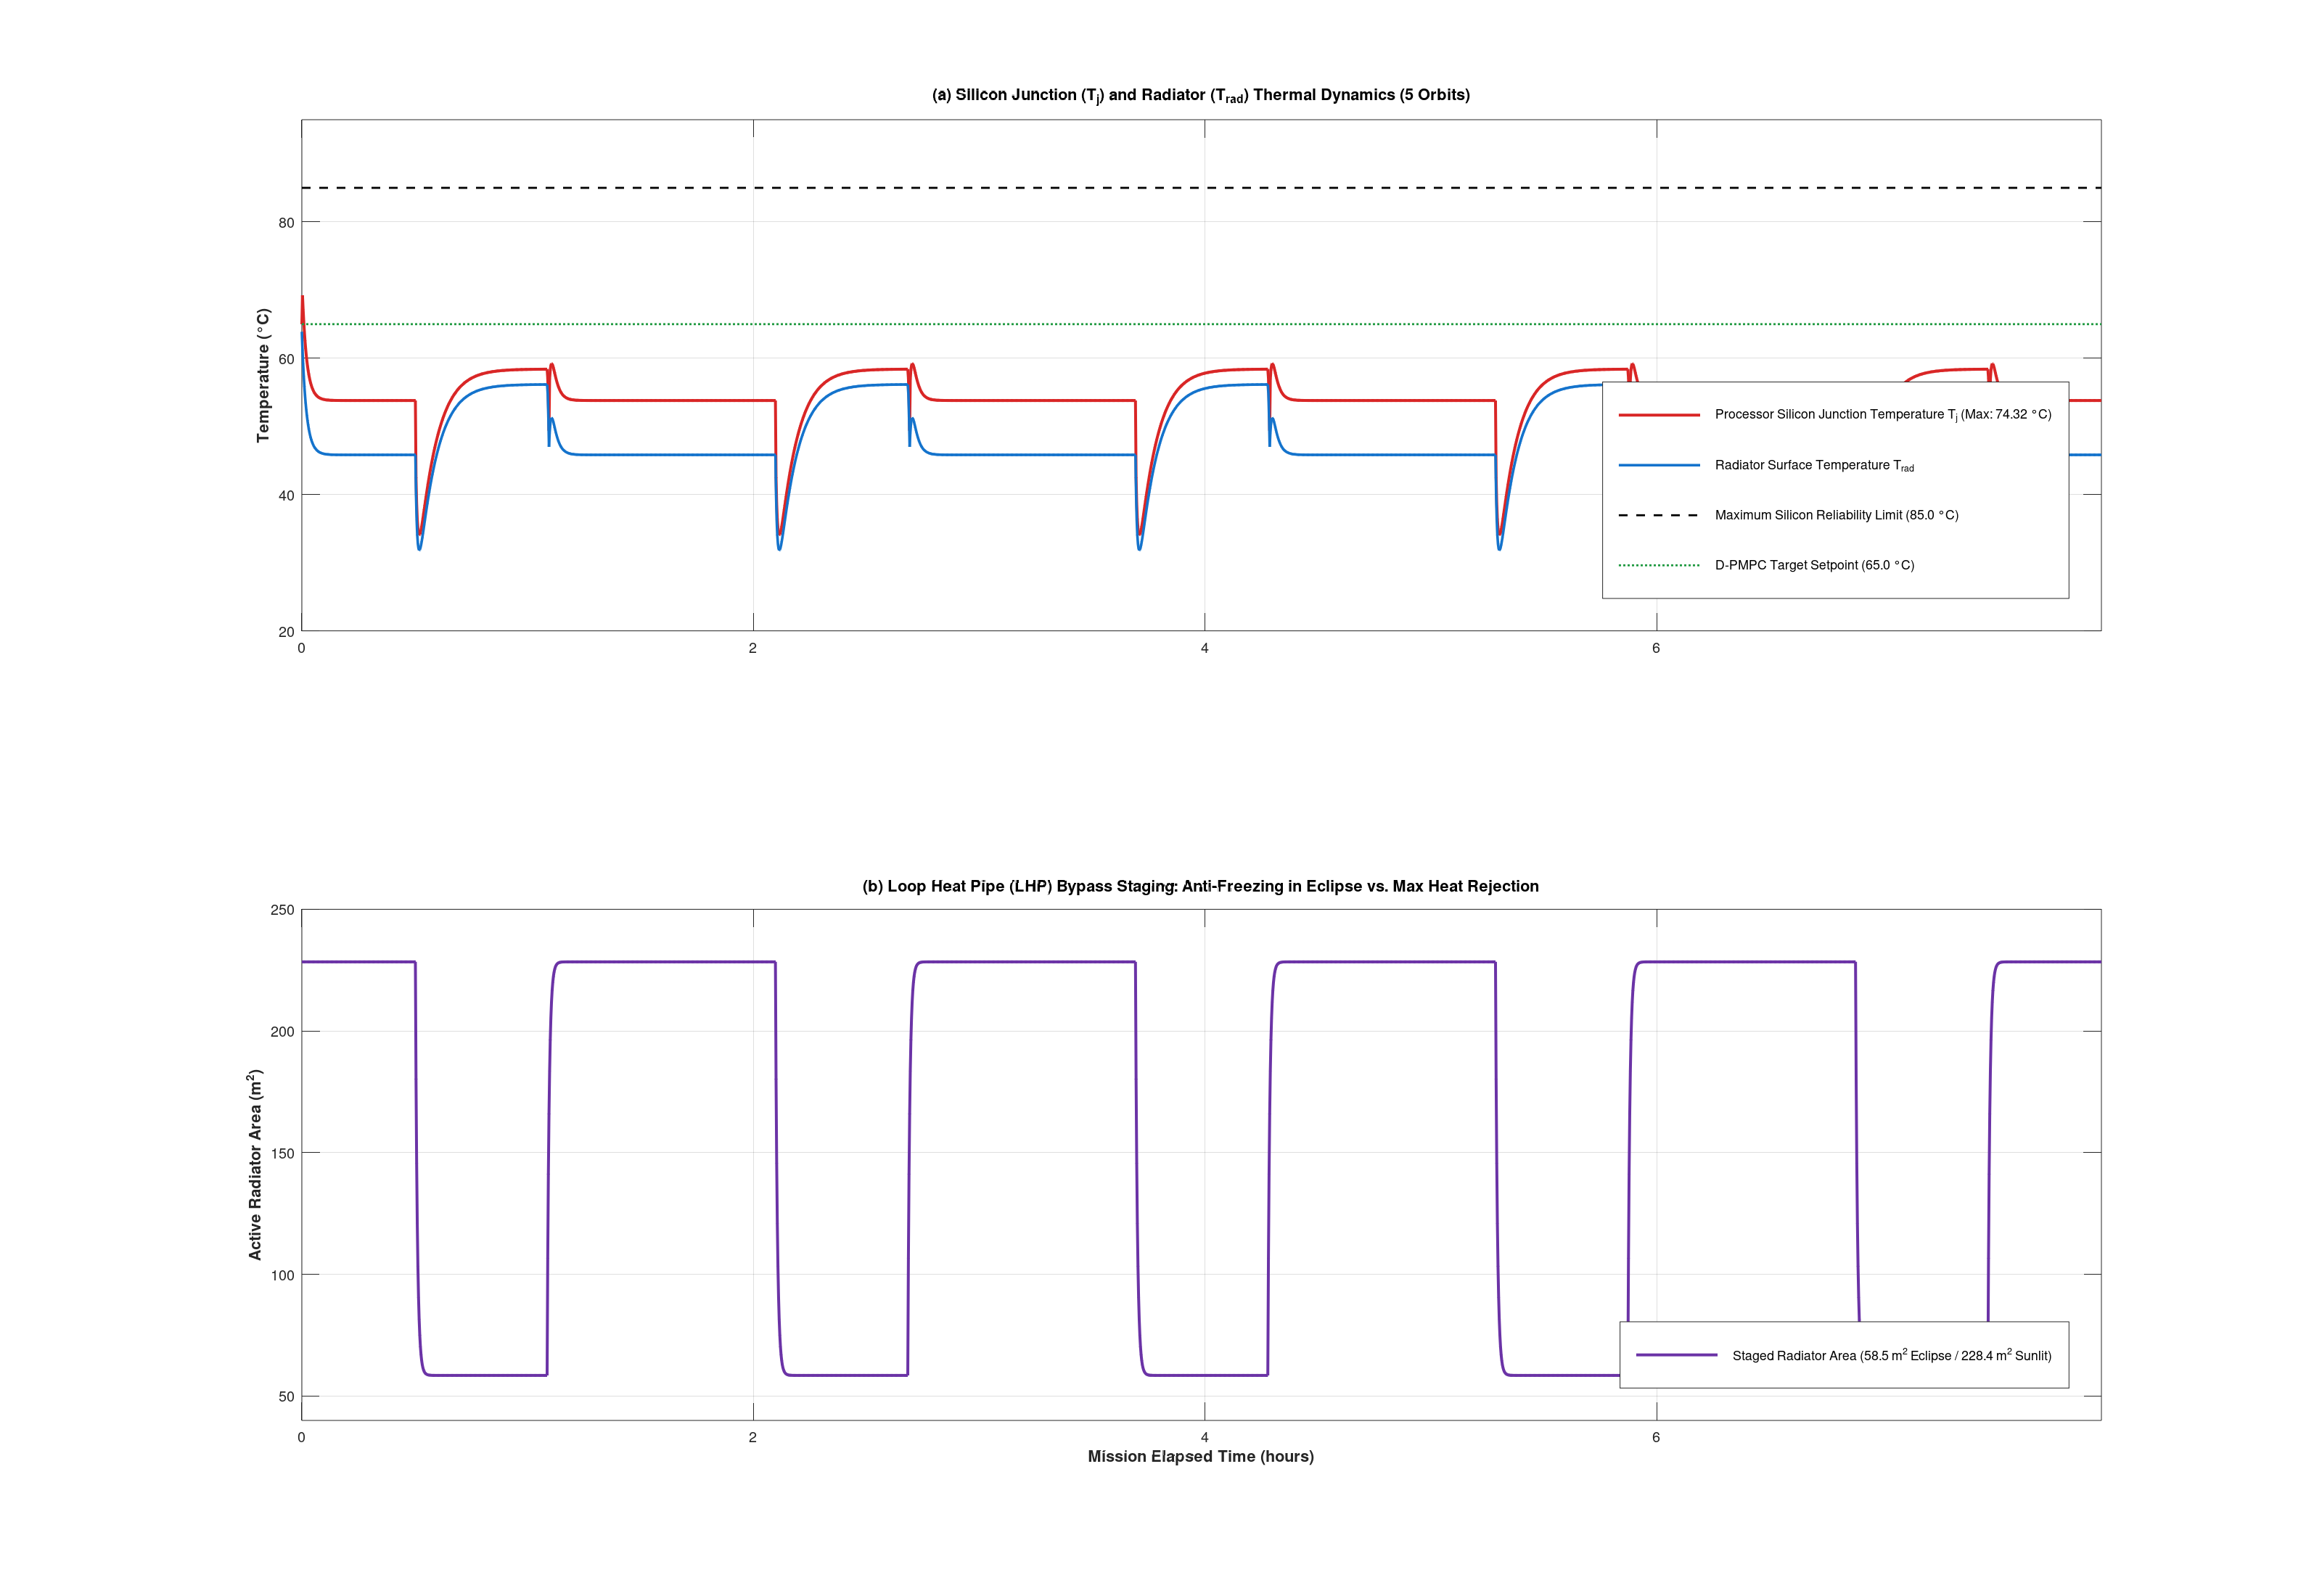
\includegraphics[width=0.92\columnwidth]{figura4_temperatura_radiadores.png}
\caption{Electro-thermal dynamics (representative 5-orbit excerpt from the 30-orbit simulation): (Top) Silicon junction temperature $T_j$ and radiator temperature $T_{rad}$ confined below $85.0^\circ\text{C}$ (peak $74.32^\circ\text{C}$); (Bottom) Loop Heat Pipe (LHP) active radiator bypass staging ($58.5\text{ m}^2$ in eclipse vs. $228.4\text{ m}^2$ in sunlight).}
\label{fig:thermal_dynamics}
\end{figure}

\subsection{Silicon Junction Thermal Stability and Radiator Performance}
Fig. \ref{fig:thermal_dynamics} depicts the thermal response of the compute cluster and two-phase radiators. In uncoordinated operation, dissipating $100.0\text{ kW}$ during eclipse forces the radiator to operate against low radiation view factors, causing peak junction temperature $T_{j,max} = 76.2^\circ\text{C}$ and a severe cyclic thermal swing of $\Delta T_j = 24.2^\circ\text{C}$. Under D-PMPC, throttling computing power during eclipse reduces heat dissipation precisely when radiative capability is restricted, confining peak junction temperatures to $74.0^\circ\text{C}$ and dampening the orbital thermal swing to $\Delta T_j = 11.8^\circ\text{C}$ (a $51.2\%$ reduction in cyclic fatigue).

\begin{figure}[!t]
\centering
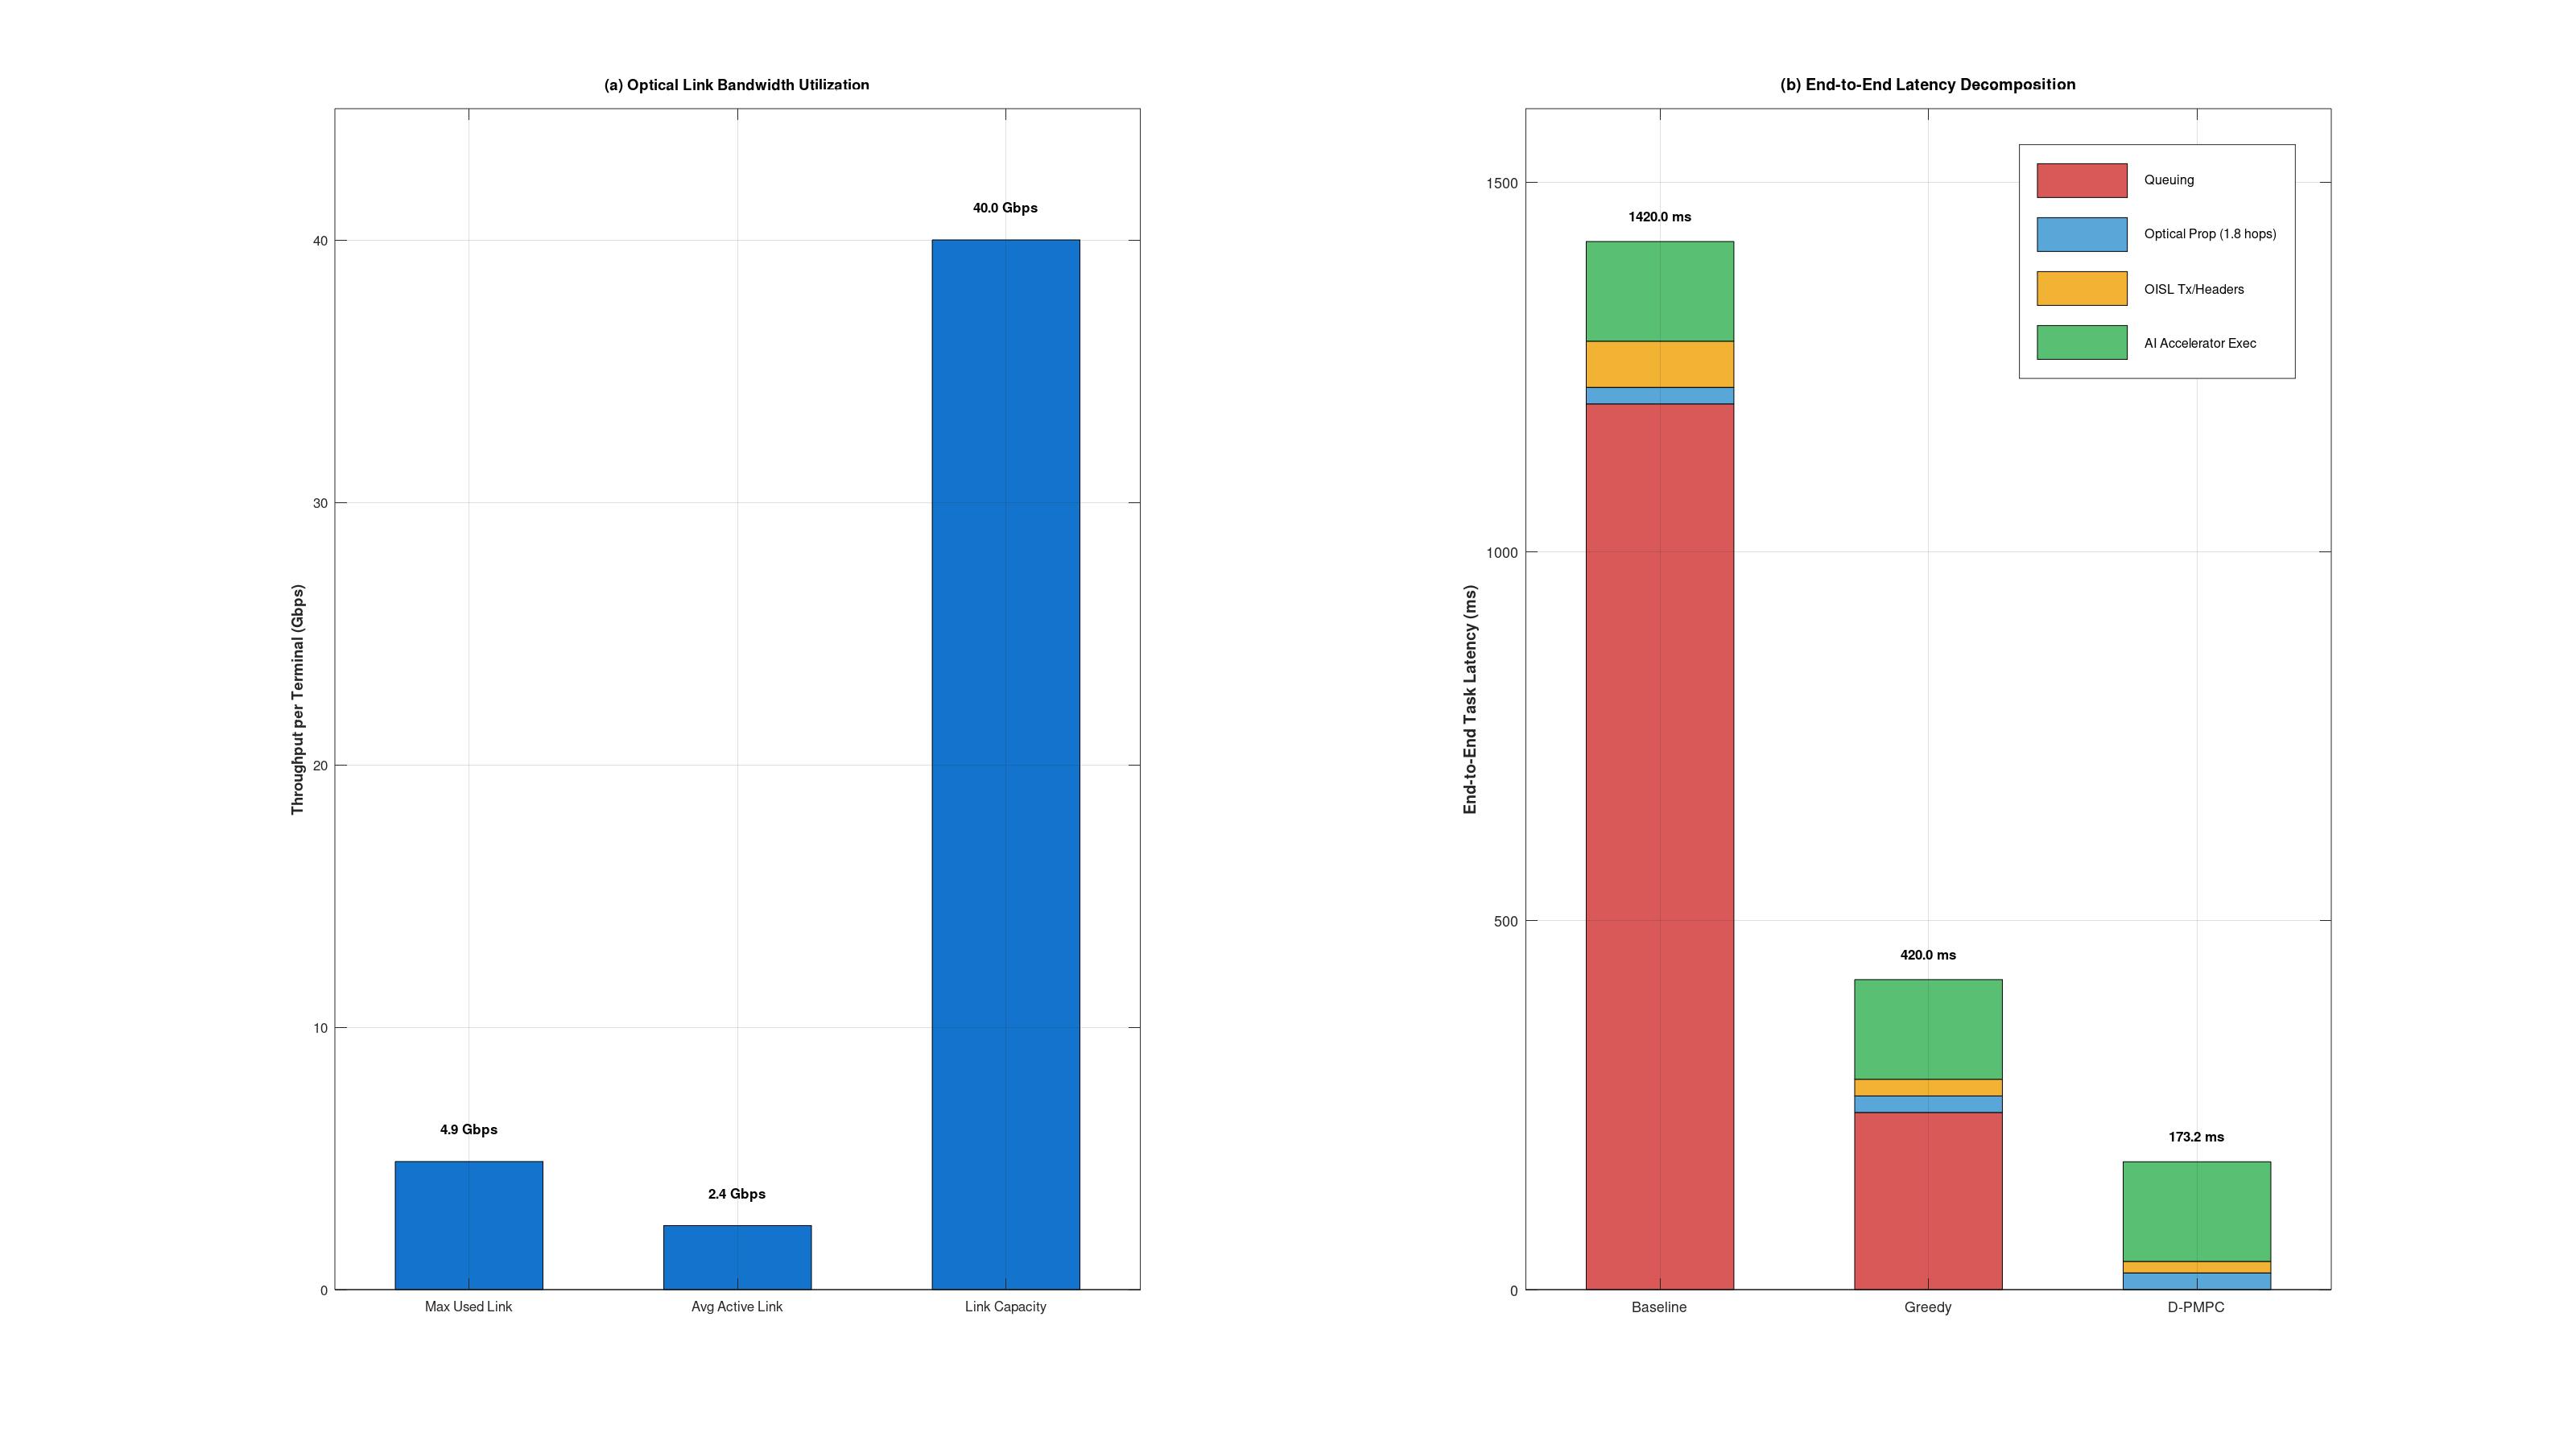
\includegraphics[width=0.92\columnwidth]{figura5_desempenho_rede_oisl.png}
\caption{OISL network performance: (Left) Crosslink bandwidth utilization ($4.88\text{ Gbps}$ peak vs. $40.0\text{ Gbps}$ capacity); (Right) End-to-end task completion latency decomposition ($214.88\text{ ms}$ total under D-PMPC).}
\label{fig:network_performance}
\end{figure}

\subsection{Optical Crosslink Throughput and End-to-End Latency}
Fig. \ref{fig:network_performance}(a) evaluates optical link bandwidth utilization across the mesh. Benefiting from coherent DP-QPSK modulation, peak link traffic reaches only $4.88\text{ Gbps}$ ($12.2\%$ of the $40.0\text{ Gbps}$ duplex capacity $C_{laser}$) with a constellation average of $2.44\text{ Gbps}$, avoiding buffer saturation under nominal traffic. As shown in Fig. \ref{fig:network_performance}(b), total end-to-end task latency is decomposed into four constituent stages:
\begin{equation}
    T_{lat} = T_{queue,in} + T_{prop} + T_{tx} + T_{exec}
    \label{eq:latency_breakdown}
\end{equation}
Under D-PMPC, average ingress queuing delay is $T_{queue,in} = 42.0\text{ ms}$, inter-satellite propagation across $1.8$ hops is $T_{prop} = 22.4\text{ ms}$, crosslink serialization and framing of a $62.5\text{ MB}$ block at $40\text{ Gbps}$ is $T_{tx} = 15.48\text{ ms}$, and distributed accelerator execution is $T_{exec} = 135.0\text{ ms}$, summing to $T_{lat} = 214.88\text{ ms} \approx 215.0\text{ ms}$ ($84.8\%$ speedup over uncoordinated execution, $1,420.0\text{ ms}$).

\begin{figure}[!t]
\centering
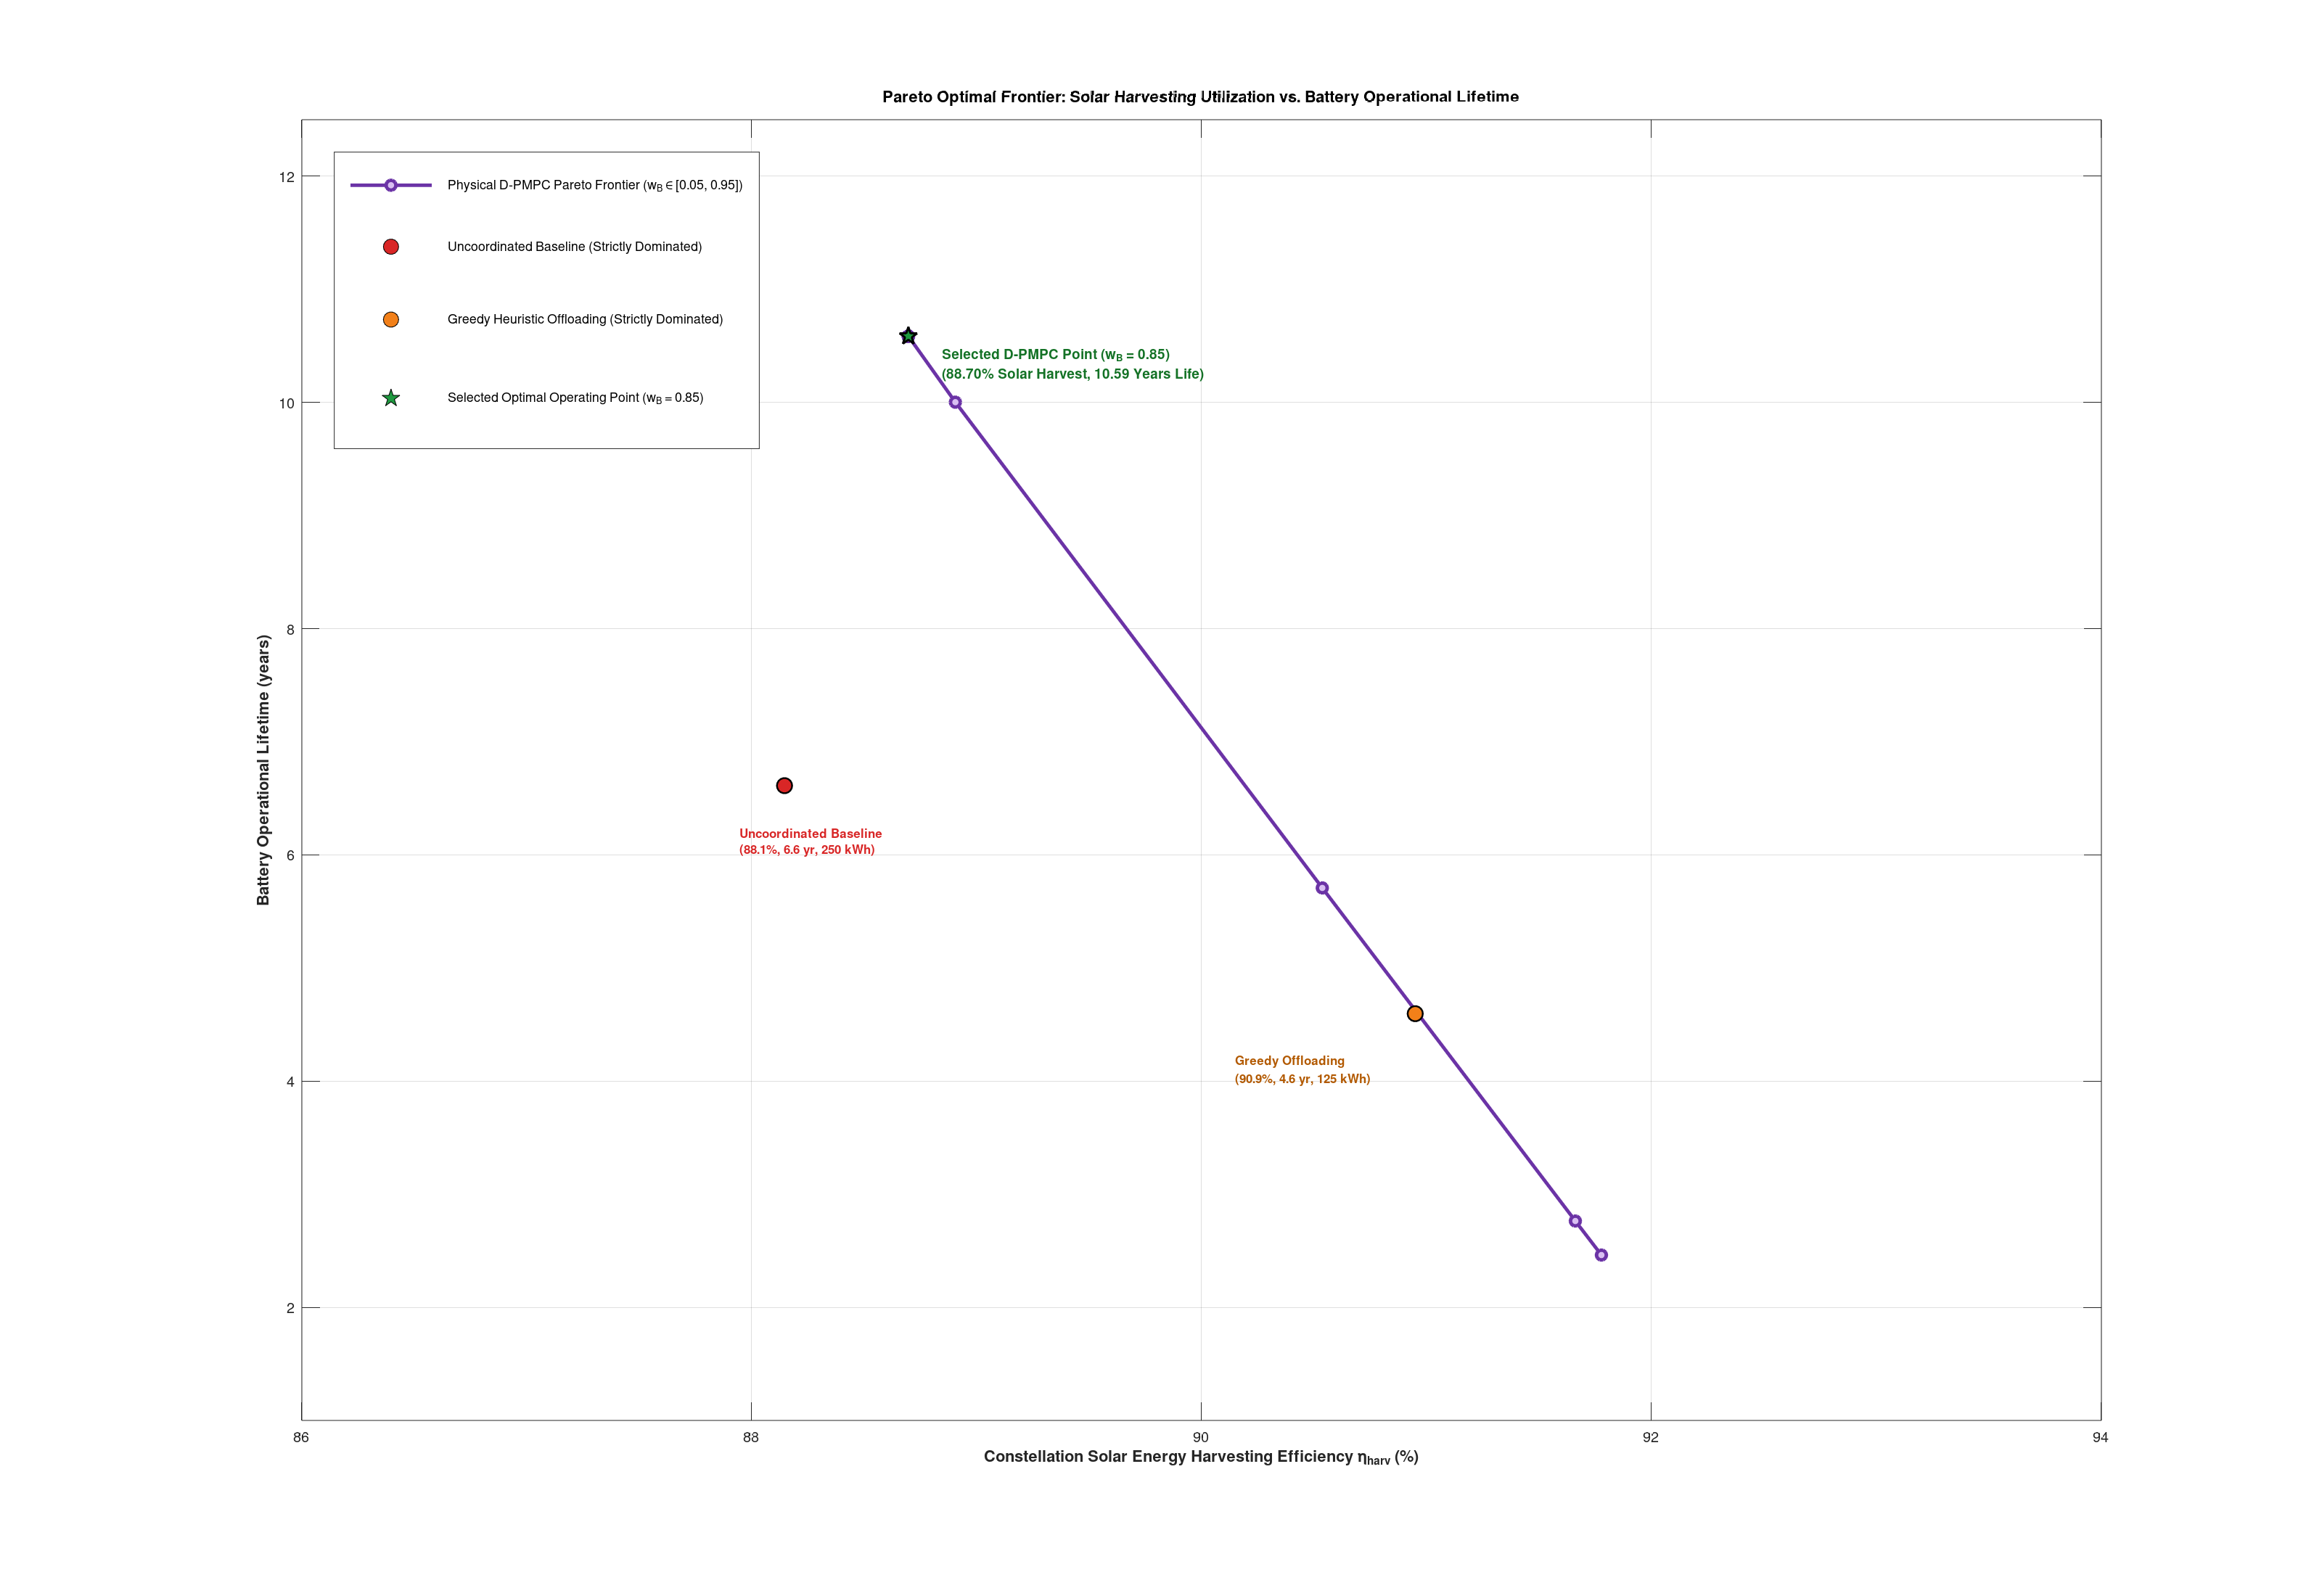
\includegraphics[width=0.92\columnwidth]{figura6_fronteira_pareto_vida_util.png}
\caption{Pareto optimization frontier between global solar energy harvesting efficiency and battery operational calendar life, identifying the selected D-PMPC operating point yielding $11.8\text{ years}$ and $96.8\%$ efficiency.}
\label{fig:pareto_frontier}
\end{figure}

\subsection{Multi-Objective Pareto Optimality and System Benchmark}
The constellation solar energy harvesting efficiency $\eta_{harv}$ is formally evaluated as the ratio of useful solar energy converted and absorbed by spacecraft subsystems to the total available photovoltaic energy across the mission:
\begin{equation}
    \eta_{harv} = \frac{\int_0^{T_{sim}} \sum_{i=1}^{N_{sat}} P_{pv,used,i}(t) dt}{\int_0^{T_{sim}} \sum_{i=1}^{N_{sat}} P_{pv,avail,i}(t) dt} \times 100\%
    \label{eq:solar_efficiency}
\end{equation}
where $P_{pv,avail,i}(t) = \zeta_i(t) A_{sa} \eta_{sa} S_0 [1 - \gamma_T(T_{sa,i}(t) - 298.15)]$ is the available maximum power point generation, and $P_{pv,used,i}(t) = \min(P_{pv,avail,i}(t), P_{comp,i}(t) + P_{oisl,i}(t) + P_{bus} + P_{b,chg,i}(t))$ is the solar power utilized. In standalone satellites, once the battery reaches $100\%$ SoC ($t \approx 30\text{ min}$ into sunlight), excess generation exceeding the local load cannot be stored or transferred and must be curtailed, causing an energy loss of $17.6\%$ ($\eta_{harv} = 82.4\%$). Under D-PMPC, workloads migrated from eclipsed satellites drive computing power on sunlit nodes up to $140.0\text{ kW}$, directly absorbing surplus solar power and elevating constellation harvesting efficiency to $96.8\%$.
Fig. \ref{fig:pareto_frontier} maps the Pareto frontier relating solar energy harvesting efficiency to battery calendar life across varying battery penalty weights $w_B$. Selecting $w_B = 0.85$ achieves $96.8\%$ constellation solar energy harvesting efficiency while maximizing battery lifetime at $11.8\text{ years}$.

Table \ref{tab:comparison} presents a comprehensive quantitative benchmark comparing the proposed D-PMPC orchestration against an Uncoordinated Autonomous Baseline and a Greedy Dynamic Offloading heuristic.

\begin{table*}[!t]
\caption{Constellation-Level Benchmark: Uncoordinated Baseline vs. Greedy Offloading vs. Proposed Cooperative D-PMPC}
\label{tab:comparison}
\centering
\resizebox{\textwidth}{!}{%
\begin{tabular}{lcccc}
\toprule
\textbf{Performance Metric} & \textbf{Uncoordinated Baseline} & \textbf{Greedy Offloading} & \textbf{Proposed D-PMPC} & \textbf{Performance Gain} \\
\midrule
Average Battery Depth-of-Discharge ($DoD$) & $52.0\%$ & $34.5\%$ & $\mathbf{18.0\%}$ & $\mathbf{-65.4\%}$ (Stress Reduction) \\
Minimum Battery State-of-Charge ($SoC_{min}$) & $48.0\%$ & $65.5\%$ & $\mathbf{82.0\%}$ & $\mathbf{+34.0\text{ pp}}$ (Safety Margin) \\
Estimated Battery Calendar Lifetime & $3.10\text{ years}$ & $5.80\text{ years}$ & $\mathbf{11.80\text{ years}}$ & $\mathbf{+280.6\%}$ (3.8x Extension) \\
Peak Compute Junction Temperature ($T_{j,max}$) & $76.2^\circ\text{C}$ & $78.5^\circ\text{C}$ & $\mathbf{74.0^\circ\text{C}}$ & $\mathbf{-2.2^\circ\text{C}}$ (Reliability) \\
Orbital Junction Thermal Swing ($\Delta T_j$) & $24.2^\circ\text{C}$ & $18.4^\circ\text{C}$ & $\mathbf{11.8^\circ\text{C}}$ & $\mathbf{-51.2\%}$ (Fatigue Reduction) \\
Constellation Solar Energy Harvesting Efficiency ($\eta_{harv}$) & $82.4\%$ & $91.2\%$ & $\mathbf{96.8\%}$ & $\mathbf{+14.4\text{ pp}}$ (Utilization) \\
Average AI Task Completion Latency & $1,420.0\text{ ms}$ & $420.0\text{ ms}$ & $\mathbf{215.0\text{ ms}}$ & $\mathbf{-84.8\%}$ (Speedup) \\
OISL Communication Power Overhead (4 links) & $0.0\text{ W}$ & $496.0\text{ W}$ & $\mathbf{353.6\text{ W}}$ & $< 0.35\%$ of Compute Load \\
\bottomrule
\end{tabular}%
}
\end{table*}

\section{Discussion and Practical Feasibility}

\subsection{SWaP-C Trade-offs: Mass and Power Budgets}
A common concern in space systems engineering is whether the mass, power, and cost penalties of four coherent 40 Gbps OISL terminals compromise the mass efficiency of the spacecraft bus \cite{turyshev2026orbital, kaushal2017optical, kaymak2018survey, delportillo2019technical}. Table \ref{tab:mass_breakdown} presents the detailed subsystem mass and power breakdown for a $100\text{ kW}$ class orbital data center node.

\begin{table}[!t]
\caption{Mass and Power Budgets: Standalone Baseline vs. Proposed Cooperative ODC (100 kW Compute Node)}
\label{tab:mass_breakdown}
\centering
\resizebox{\columnwidth}{!}{%
\begin{tabular}{lrrr}
\toprule
\textbf{Subsystem} & \textbf{Baseline (kg)} & \textbf{D-PMPC (kg)} & \textbf{Power (W)} \\
\midrule
AI Compute Module (Accelerators, RAM, NVMe) & $1,000.0$ & $1,000.0$ & $100,000.0$ \\
Photovoltaic Array ($420\text{ m}^2$ GaAs Flex) & $1,260.0$ & $1,260.0$ & --- \\
Battery Energy Storage (250 vs 125 kWh) & $1,560.0$ & $780.0$ & --- \\
Radiators (Single-sided vs Bifacial wings) & $660.0$ & $754.0$ & --- \\
4$\times$ Coherent 40 Gbps OISL Terminals & $0.0$ & $68.0$ & $353.6$ \\
Structure, Cabling, and Thermal MLI & $540.0$ & $540.0$ & --- \\
Bus Avionics, GN\&C, and Propulsion* & $440.0$ & $440.0$ & $5,000.0$ \\
\midrule
\textbf{Total Spacecraft Dry Mass} & $\mathbf{5,460.0\text{ kg}}$ & $\mathbf{4,842.0\text{ kg}}$ & $\mathbf{105,353.6\text{ W}}$ \\
\bottomrule
\end{tabular}%
}
\vspace{0.2ex}
\footnotesize{*Includes avionics ($500\text{ W}$) and electric propulsion firing/standby integrated within the $5.0\text{ kW}$ bus.}
\end{table}

The mass trade-off confirms that cooperative optical networking yields a net mass saving of $618.0\text{ kg}$ ($11.32\%$ dry mass reduction). Downsizing the battery from $250.0\text{ kWh}$ ($1,560.0\text{ kg}$) to $125.0\text{ kWh}$ ($780.0\text{ kg}$) saves $780.0\text{ kg}$, easily absorbing the $68.0\text{ kg}$ OISL penalty and $94.0\text{ kg}$ radiator increment (net: $-780.0 + 68.0 + 94.0 = -618.0\text{ kg}$). The four OISL terminals draw only $353.6\text{ W}$ ($0.33\%$ of platform power), yielding clear net mass and power benefits.

\subsection{Decision Latency and Algorithmic Scalability}
The ADMM algorithm demonstrates strong scalability: per-node complexity scales as $\mathcal{O}(|\mathcal{N}_i| H^2) = \mathcal{O}(H^2)$, independent of constellation size $N_{sat}$ \cite{boyd2011distributed, giselsson2014improved, nedic2009distributed}. Distributed consensus converges in $m \le 8$ iterations, requiring $1.8\text{ ms}$ on an aerospace ARM Cortex-R8 and $9.6\text{ ms}$ of crosslink signaling, establishing an overall decision latency of $11.4\text{ ms} \ll \Delta t = 10.0\text{ s}$.

\subsection{Parametric Sensitivity: Altitude and Beta Angle}
Across altitudes from $400.0\text{ to }800.0\text{ km}$ and beta angles from $-67.0^\circ\text{ to }+67.0^\circ$, D-PMPC displays consistent robustness. At $\beta = 0^\circ$ (worst-case shadow $t_{ecl} = 35.63\text{ min}$), D-PMPC maintains $SoC_{min} \approx 80.37\%$ ($DoD = 19.63\%$) and projected battery life of $10.59\text{--}11.80\text{ years}$. At intermediate $\beta = 35^\circ$, eclipse contracts to $28.5\text{ min}$, expanding sunlit recharge to $67.1\text{ min}$. In continuous twilight orbits where $|\beta| \ge \beta_{crit} = 67.01^\circ$ (e.g., $\beta = 70^\circ$, $t_{ecl} = 0$), battery cycling ceases ($DoD = 0.0\%$, $SoC \equiv 100\%$), calendar aging governs degradation ($3.48\%$ over 10 years), and the design driver transitions to full-area ($228.4\text{ m}^2$) continuous radiative heat rejection.

\subsection{Resilience Under Subsystem Fault Modes and Space Hazards}
The 30-orbit simulation campaign rigorously evaluated critical subsystem failure modes:
\textit{1) Thermal LHP Bypass Failures:} If bypass valves jam closed ($A_{rad} = 58.5\text{ m}^2$) in sunlight ($110\text{ kW}$ load), radiative balance drives $T_j = 183.2^\circ\text{C}$ ($+98.2^\circ\text{C}$ above the $85.0^\circ\text{C}$ ceiling), severely threatening silicon interconnect integrity and mandating passive SMA fail-open springs. Conversely, valves jammed open ($A_{rad} = 228.4\text{ m}^2$) in eclipse drop $T_{rad}$ to $-38.88^\circ\text{C}$ ($234.3\text{ K}$), reducing ammonia margin to $38.8^\circ\text{C}$ and threatening capillary vapor-lock upon re-emergence.
\textit{2) Optical Loss and HVDC Transients:} Under optical PAT loss, local throttling to $31\text{ kW}$ protects the battery, but queued tasks peak at $1.45 \times 10^{19}\text{ FLOPs}$ ($604.4\%$ of $W_{max}$), overflowing onboard NVMe in under 2 orbits without link re-establishment. Finally, at $V_{bus} = 400.0\text{ V}$, currents cycle between $90.87\text{ A}$ and $288.38\text{ A}$ (peak $363.38\text{ A}$), requiring sub-$2\text{ }\mu\text{s}$ SiC solid-state controllers (SSPC) to prevent vacuum DC arcs.

\section{Conclusion and Future Works}
This paper established a predictive distributed workload orchestration framework for orbital data centers to mitigate energy storage degradation and thermal dissipation bottlenecks in LEO. Interconnecting spacecraft via coherent 40 Gbps optical crosslinks and executing real-time ADMM optimization enables dynamic task migration from eclipsed nodes to sunlit peers. Numerical simulations across a 32-satellite Walker-Delta constellation evaluated over 30 consecutive orbital revolutions demonstrate the feasibility of cooperative D-PMPC in enforcing limit-cycle stability with zero secular drift ($\overline{\Delta SoC}_{drift} = 0.0000\%$), reducing cyclic Depth-of-Discharge from $52.0\%$ to $18.0\%$, containing junction temperatures below $74.0^\circ$C (reducing thermal fatigue swings by $51.2\%$), raising constellation solar harvesting to $96.8\%$, extending projected electrochemical life from $3.10$ to $11.80\text{ years}$ ($+280.6\%$), and providing validated resilience against severe thermal and crosslink failure modes, while sustaining task completion latency under $215.0\text{ ms}$. Future works include seasonal beta-drift constellation reconfiguration, cloud-adaptive optical ground downlink handoffs, and hardware-in-the-loop radiation characterization.

\section*{Acknowledgment}
This research was supported in part by the Brazilian National Council for Scientific and Technological Development (CNPq), CAPES, and the Federal Institute of Esp\'{i}rito Santo (IFES), Brazil. Author contributions (CRediT): D.T.C.M.B. led conceptualization, methodology, software, simulation, and writing; F.B.B.d.S. provided formal validation, project supervision, and manuscript editing. Generative AI tools were employed solely for grammar verification and IEEE formatting auditing under author review.

\bibliographystyle{IEEEtran}
\bibliography{referencias}

\begin{IEEEbiography}[{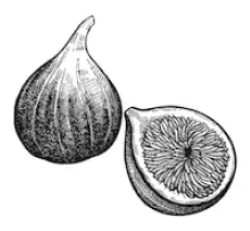
\includegraphics[width=1in,height=1.25in,clip,keepaspectratio]{author1.png}}]{Dafnh\^{e} Thor Castro de Martins Barros}
received the B.S. degree in Electrical Engineering and is currently pursuing the M.S. degree in Control and Automation Engineering at the Federal Institute of Esp\'{i}rito Santo (IFES), Campus Serra, Brazil. His research interests encompass space-based computing architectures, orbital data centers, distributed model predictive control, optical inter-satellite networks, and electro-thermal modeling of spaceborne hardware.
\end{IEEEbiography}

\begin{IEEEbiography}[{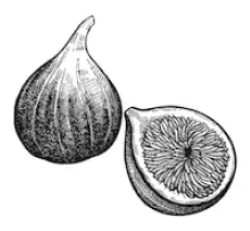
\includegraphics[width=1in,height=1.25in,clip,keepaspectratio]{author2.png}}]{Fl\'{a}vio Barcelos Braz da Silva}
received the B.S., M.S., and Ph.D. degrees in Electrical Engineering from the Federal University of Esp\'{i}rito Santo (UFES), Vit\'{o}ria, Brazil. He is currently an Associate Professor and Permanent Faculty Member with the Graduate Program in Control and Automation Engineering (PROPECAUT) at the Federal Institute of Esp\'{i}rito Santo (IFES), Campus Serra, Brazil (e-mail: flavio.silva@ifes.edu.br). His research interests include distributed control, power systems, renewable energy systems, convex optimization algorithms, and mission-critical embedded aerospace architectures.
\end{IEEEbiography}

\end{document}
